\documentclass[12pt]{ociamthesis}  % default square logo 
%\documentclass[12pt,beltcrest]{ociamthesis} % use old belt crest logo
%\documentclass[12pt,shieldcrest]{ociamthesis} % use older shield crest logo

%load any additional packages
\usepackage{amssymb}
\usepackage{listings}

\usepackage{color}
 
\definecolor{codegreen}{rgb}{0,0.6,0}
\definecolor{codegray}{rgb}{0.5,0.5,0.5}
\definecolor{codepurple}{rgb}{0.58,0,0.82}
\definecolor{backcolour}{rgb}{0.95,0.95,0.92}
 
\lstdefinestyle{mystyle}{
    backgroundcolor=\color{backcolour},   
    commentstyle=\color{codegreen},
    keywordstyle=\color{magenta},
    numberstyle=\tiny\color{codegray},
    stringstyle=\color{codepurple},
    basicstyle=\footnotesize,
    breakatwhitespace=false,         
    breaklines=true,                 
    captionpos=b,                    
    keepspaces=true,                 
    numbers=left,                    
    numbersep=5pt,                  
    showspaces=false,                
    showstringspaces=false,
    showtabs=false,                  
    tabsize=2,
    language=python
}
 
\lstset{style=mystyle}

%input macros (i.e. write your own macros file called mymacros.tex 
%and uncomment the next line)
%\include{mymacros}

\title{Laporan \\[1ex]     %your thesis title,
        Database II}   %note \\[1ex] is a line break in the title

\author{Alvian Daniel Sinaga}             %your name
\college{\textbf{1.18.4.077\\[5ex]
}  }

\degree{\textbf{POLITEKNIK POS INDONESIA}}     %the degree
\degreedate{\textbf{BANDUNG 2019}}         %the degree date

%end the preamble and start the document
\begin{document}

%this baselineskip gives sufficient line spacing for an examiner to easily
%markup the thesis with comments
\baselineskip=18pt plus1pt

%set the number of sectioning levels that get number and appear in the contents
\setcounter{secnumdepth}{3}
\setcounter{tocdepth}{3}


\maketitle                  % create a title page from the preamble info
\begin{dedication}

”Pendidikan adalah paspor untuk masa,untuk hari esok yang dimiliki oleh orang yang mempersiapkan hari ini. \\
(Malcolm X) \\
Barangsiapa tidak mau merasakan pahitnya belajar, ia akan merasakan hinanya kebodohan sepanjang hidupnya, \\ 
(imam Syafi'i rahimahullah) \\

\end{dedication}        % include a dedication.tex file
\begin{acknowledgements}
\par
Assalamualaikum warahmatullahi wabarakatuh. Segala puji bagi Allah SWT yang telah melimpahkan rahmat dan hidayah-Nya, sehingga kami dapat menyelesaikan laporan dengan judul “Laporan Pembelajaran Oracle Academy Virtual Students Day”. Penyusunan laporan ini dimaksudkan untuk memenuhi tugas D4 teknik informatika pada bidang mata kuliah Database II. Dalam penyusunan laporan ini, kami mengucapkan kepada pihak yang telah membantu atau membimbing kami dalam penyusunan laporan ini ini. Laporan ini juga tidak terlepas dari bapak Syafrial Fachri Pane, S.T., M.T.I selaku dosen matakuliah database. Penulis telah membuat laporan ini dengan sebaik-baiknya, diharapkan memberikan kritik dan saran dari semua pihak yang bersifat membangun, terimakasih.

\begin{raggedleft}




\vspace{12ex}
Bandung, 17 Oktober 2019

\vspace{6ex}
Penulis

\end{raggedleft}

\end{acknowledgements}   % include an acknowledgements.tex file
\begin{abstract}
	Panduan Penulisan Jurnal Ilmiah (PPJI) ini dibuat dengan tujuan memberikan acuan bagi para sivitas akademika
	yang memulai menulis jurnal ilmiah. Pada intinya PPJI menjelaskan secara lengkap tentang standar pengerjaan jurnal internasional dari pengalaman penulisan dari tahun 2017. Di dalamnya memuat aturan standar penulisan dan penggunaan Latex sebagai editor. Dengan demikian diharapkan semua sivitas akademika dapat membuat jurnal ilmiah dengan
	 lancar dan sesuai dengan standar.
\end{abstract}          % include the abstract

\begin{romanpages}          % start roman page numbering
\tableofcontents            % generate and include a table of contents
\listoffigures              % generate and include a list of figures
\end{romanpages}            % end roman page numbering

%now include the files of latex for each of the chapters etc
\chapter{Oracle Aplication Express}


\section{Pengertian Oracle APEX}
Oracle Aplication Express\cite{OracleApex}. Adalah sebuah wadah dan sarana untuk membuat aplikasi yang menggunakan database Oracle Itu sendiri, pada kelas Online pertama saya belajar banyak hal cara Menggunakan Aplikasi Oracle Apex online yang di dalam video sudah diberikan link diantaranya Request Workspace, Create Workspace, Membuat Spreadsheet Pertama.

\section{Cara Membuat Aplikasi Sederhana di Apex Oracle Online}
Langkah - langkahnya adalah sebagai berikut :
\begin{enumerate}
    \item Melakukan registrasi untuk masuk pada apex . di tampilan ini user memasukkan nama workspace yang telah dibuat serta memasukkan username dan password. ketika user belum mempunyai workspace . maka user mengklik request a workspace untuk membuat workspace baru .
\newline
    \item   Lalu request a workspace dengan mengisikan first name, last name
    , email dan membuat workspace . kemudian klik next 
\newline
    \item   verifikasi memlalui email . buka email lalu klik pesan dari oracle kemudian klik clik create workspace .
\newline
    \item   Masukkan oracle application express dengan memasukkan nama workspace , masukkan nama user dan password lalu klik sign in
\newline
    \item  Akan keluar tampilan seperti gambar yang sudah terlampir pada platform
    \newline
    \begin{figure} [!htbp]
        \centering
        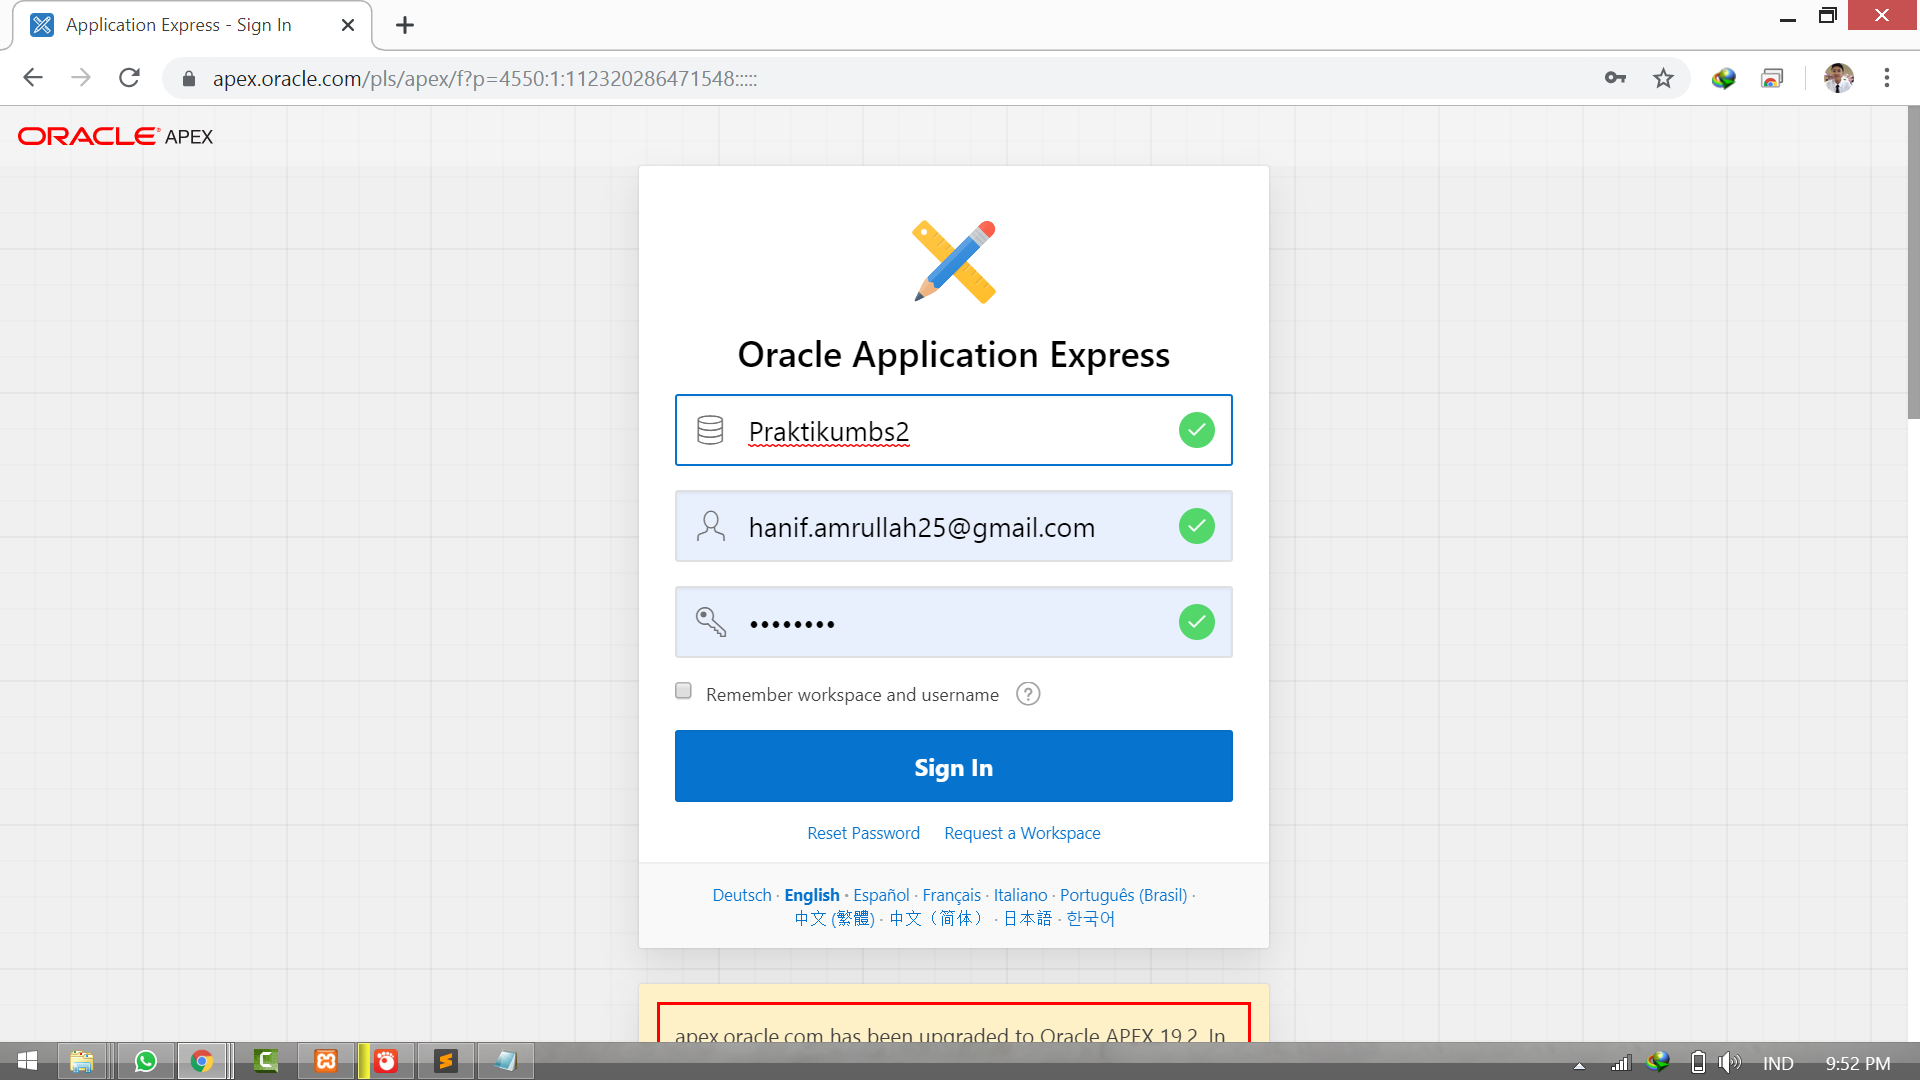
\includegraphics[scale=0.5]{figures/1.png}
        \caption{Create}
        \label{penanda}
    \end{figure}
\newline
    \item  lalu create
\newline
    \item  Setelah itu unggah file dalam bentuk csv,xlxs,xml atau json .
    \newline
    \begin{figure}[!htbp]
        \centering
        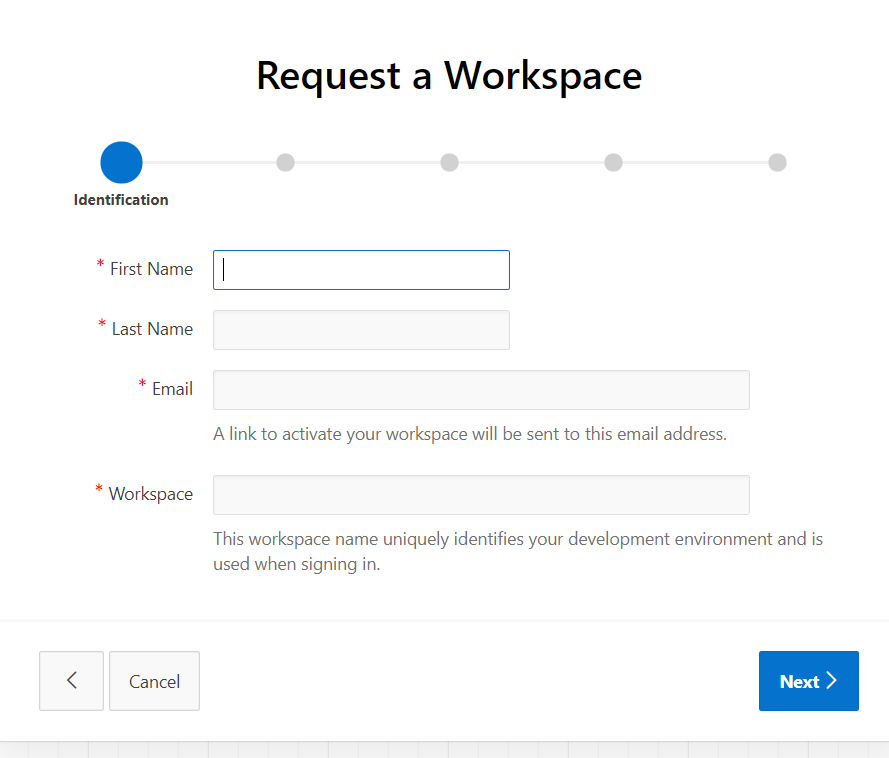
\includegraphics[scale=0.5]{figures/3.png}
        \caption{Memasukan file}
        \label{penanda}
    \end{figure}
\newline
    \item  Kemudian pilih file data excel yang telah dibuat dalam bentuk xlsx
\newline
    \item  Buat tabel dengan memasukkan nama tabel disini saya membuat tabel Mahasiswa terlebih dahulu .
    \newline
    \begin{figure}[!htbp]
        \centering
        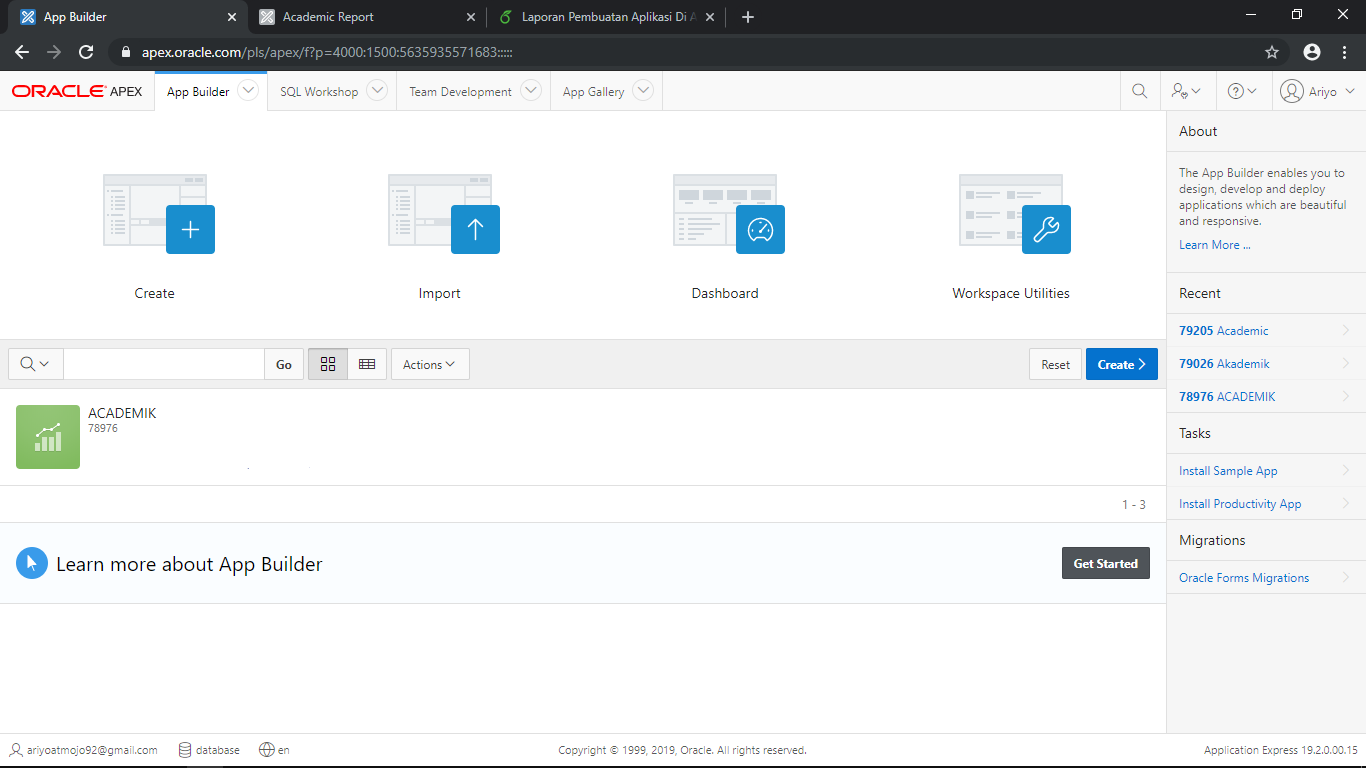
\includegraphics[scale=0.5]{figures/4.png}
        \caption{Membuat nama tabel Mahasiswa}
        \label{fig:my_label}
    \end{figure}
\newline
    \item Klik configure untuk mengecek apakah tabel dari data excel sudah benar atau tidak 
\newline
    \item  Lalu scroll kebawah sehingga keluar daftar nama mahasiswa yang berada pada file excel kemudian klik load data 
\newline
    \item Kemudia klik X untuk membuat tabel berikutnya , lakukan seperti perintah yang diatas lagi . selanjutnya membuat tabel dosen 
\newline
    \begin{figure}[!htbp]
        \centering
        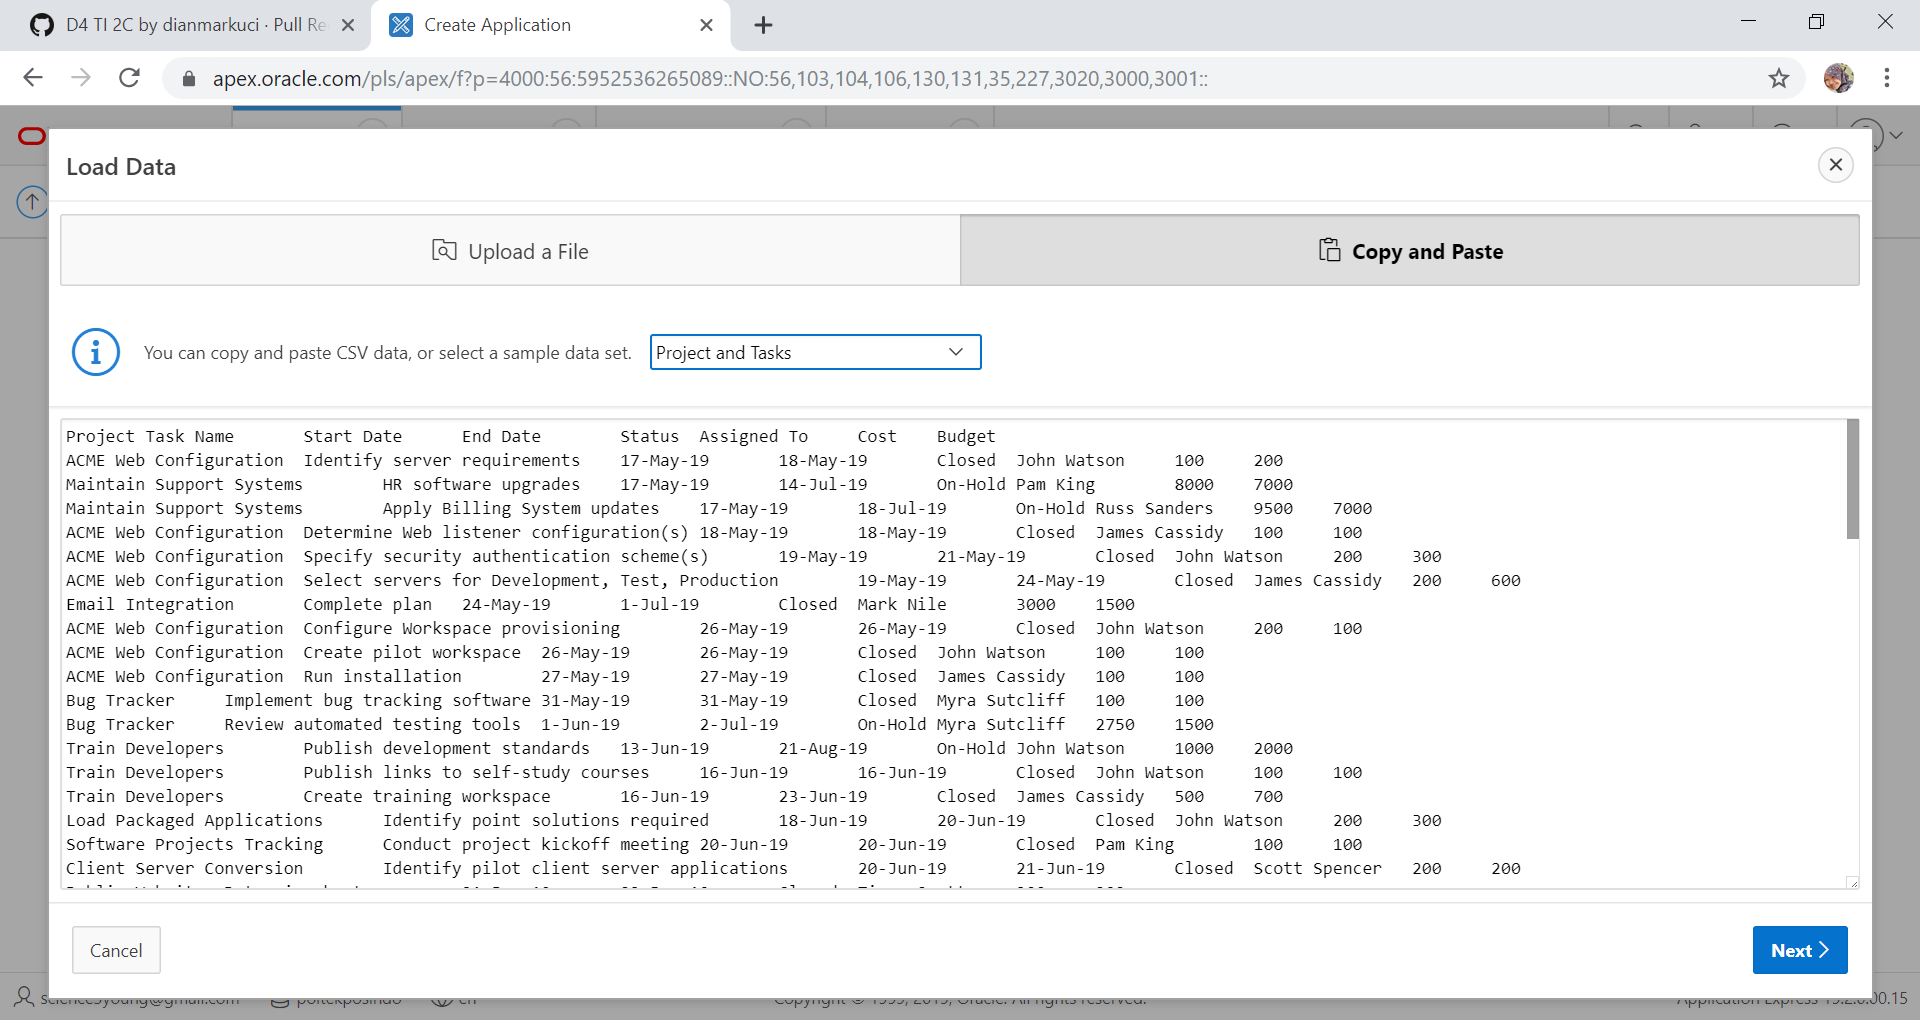
\includegraphics[scale=0.5]{figures/7.png}
        \caption{Membuat nama tabel dosen}
        \label{fig:my_label}
    \end{figure}
\newline
    \item Lalu configure dan klik load data , lalu klik X untuk keluar .
    \newline
    \item Kemudian membuat tabel Kuliah .
    \begin{figure}[!htbp]
        \centering
        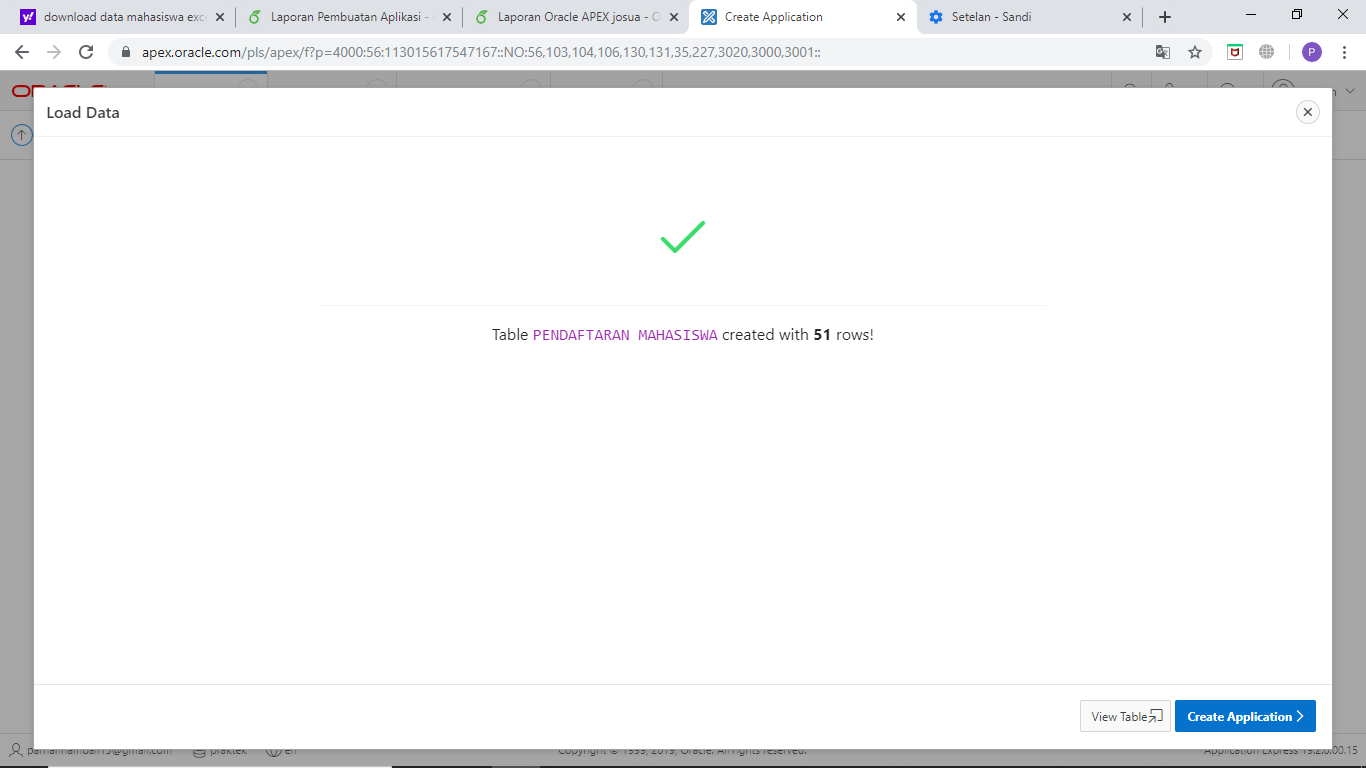
\includegraphics[scale=0.5]{figures/8.png}
        \caption{Membuat nama tabel kuliah}
        \label{fig:my_label}
    \end{figure}
    \newline
    \item Lakukan lagi perintah seperti diatas sampai semua tabel selesai dibuat . setelah tabel kuliah membuat tabel jadwal .
    \newline
    \begin{figure}[!htbp]
        \centering
        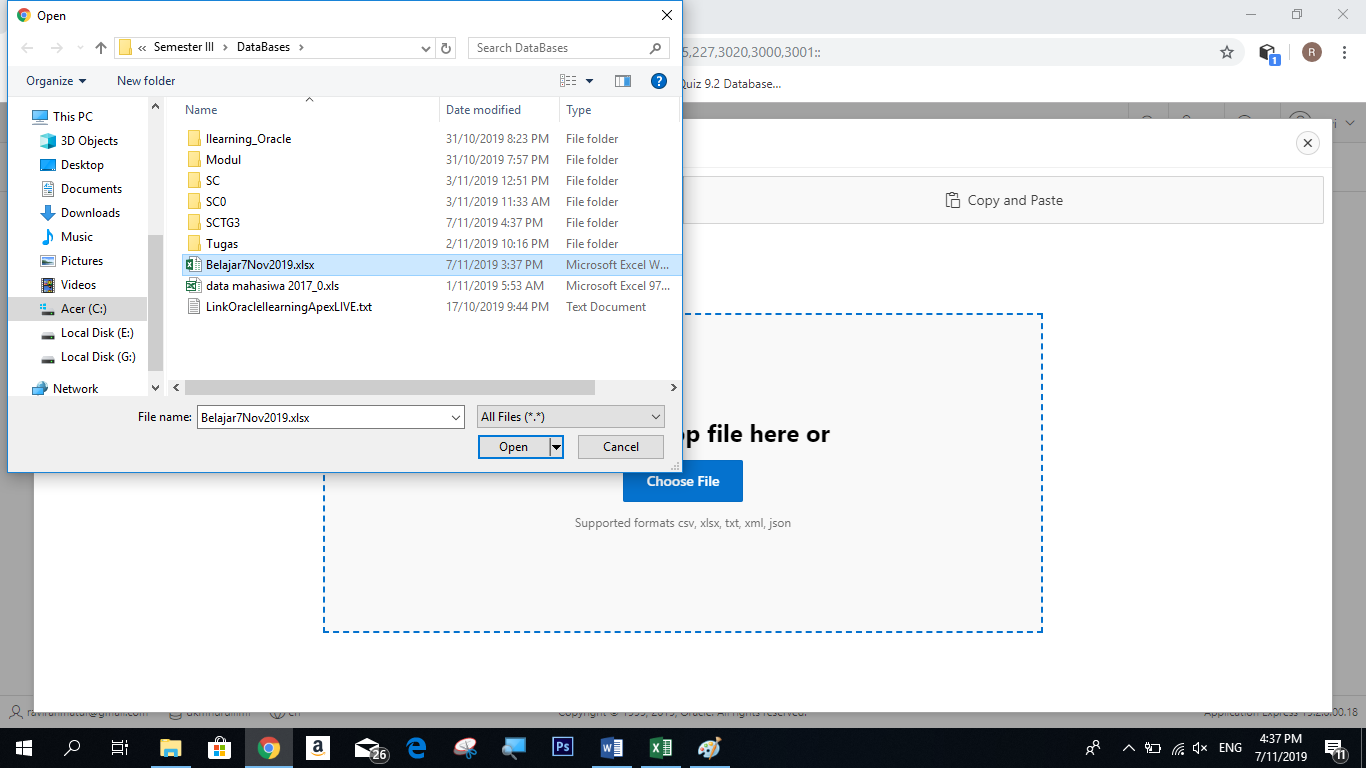
\includegraphics[scale=0.5]{figures/9.png}
        \caption{Membuat nama tabel jadwal}
        \label{fig:my_label}
    \end{figure}
    \newline
    \item Membuat tabel nilai . 
    \newline
    \begin{figure}[!htbp]
        \centering
        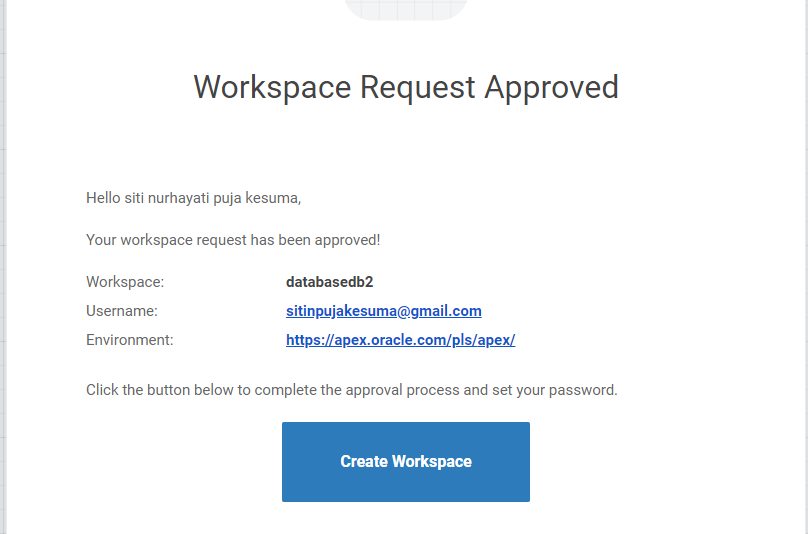
\includegraphics[scale=0.5]{figures/10.png}
        \caption{Mmebuat nama tabel nilai}
        \label{fig:my_label}
    \end{figure}
    \newline
    \item  Tampilan selanjutnya adalah create lalu hapus ID disetiap tabel .
\newline
\begin{figure}[!htbp]
    \centering
    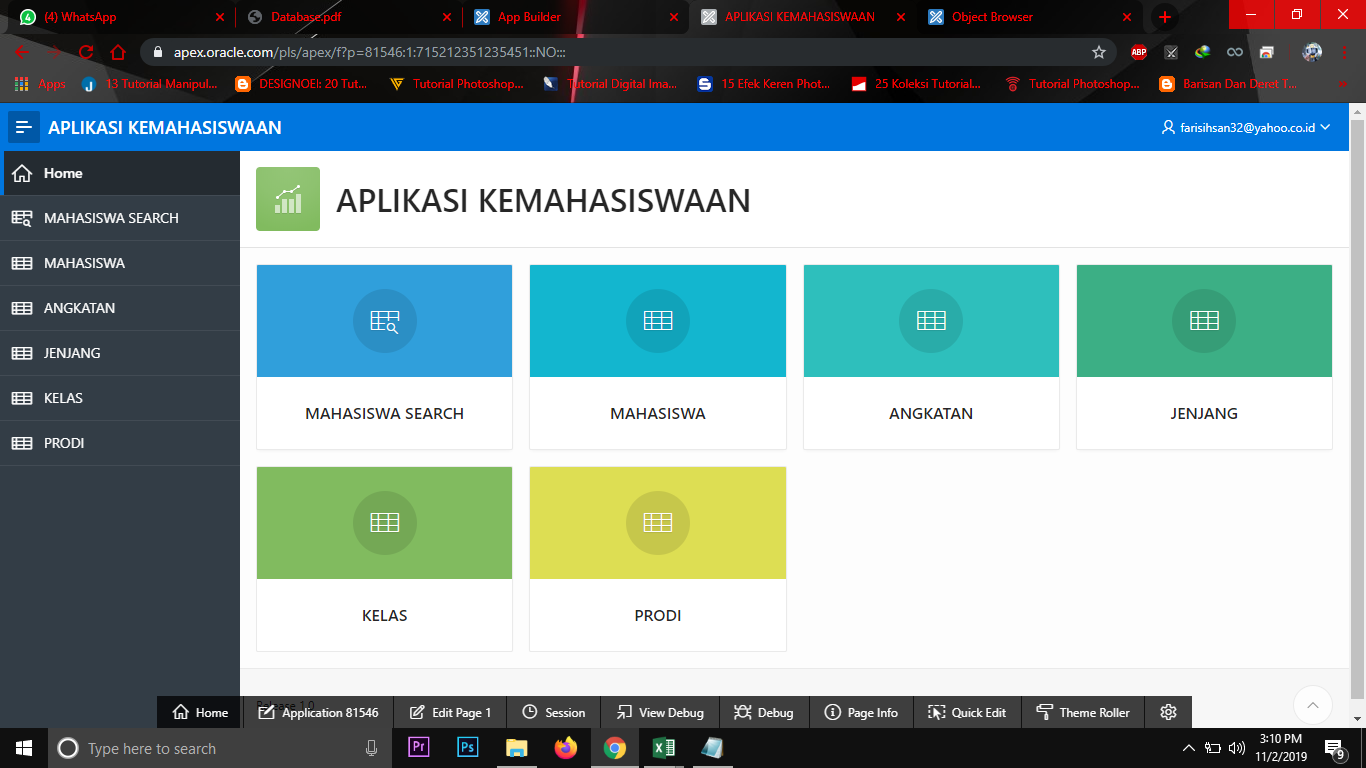
\includegraphics[scale=0.5]{figures/12.png}
    \caption{Menghapus ID}
    \label{fig:my_label}
\end{figure}
\newline
\item Lalu ubah setaip tabel ke primary dan foreign key , pertama kita ubah terlebih dahulu yang primary seperti Dosen , Mahasiswa dan kuliah sedangan jadwal dan nilai kita ubah ke foreign key .
\newline
\begin{figure}[!htbp]
    \centering
    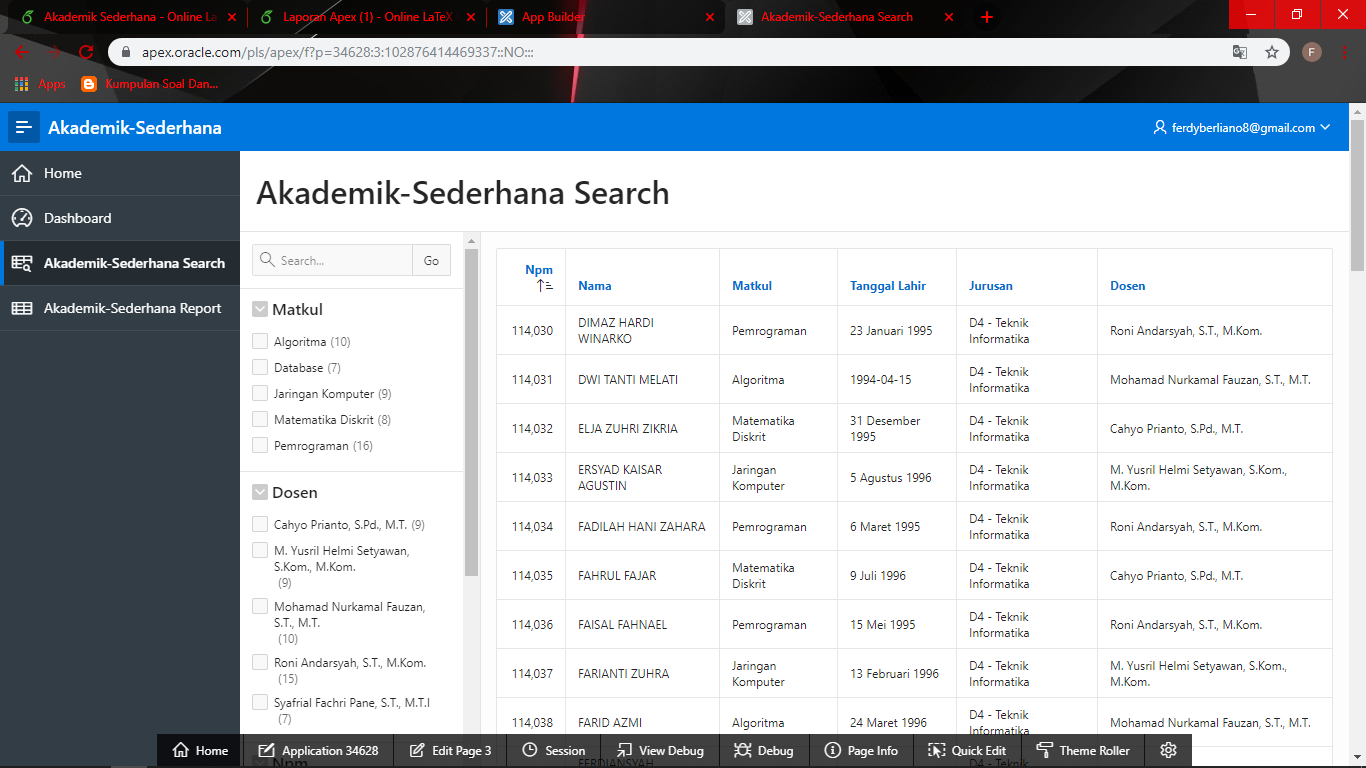
\includegraphics[scale=0.3]{figures/20.png}
    \caption{Mengubah tabel menjadi primary dan foreign key}
    \label{fig:my_label}
\end{figure}
\newline
\item Setelah itu kita buka app builder dan create .
\newline
\begin{figure}[!htbp]
    \centering
    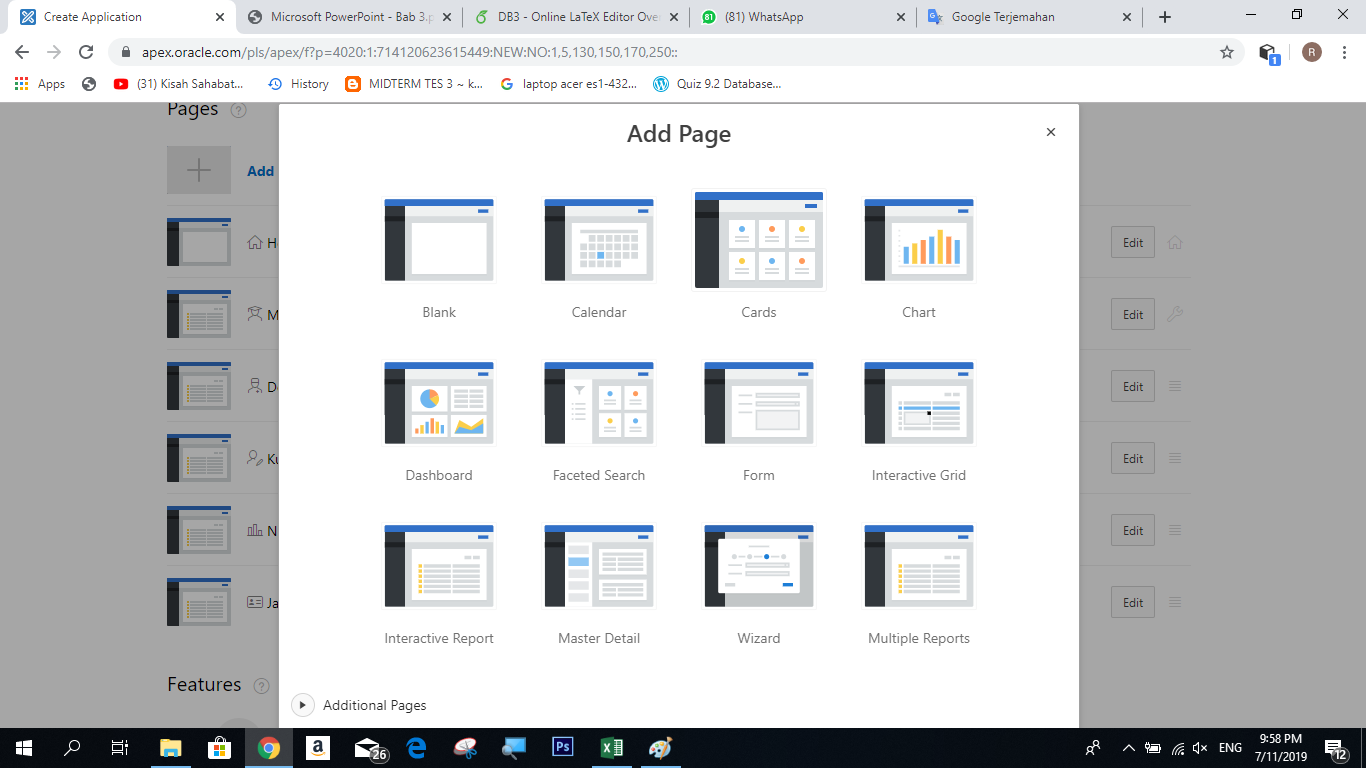
\includegraphics[scale=0.5]{figures/24.png}
    \caption{App Builder}
    \label{fig:my_label}
\end{figure}
\newline
\item Kemudian add page untuk memilih fitur apa saja yang mau digunakan . 
\newline
\begin{figure}[!htbp]
    \centering
    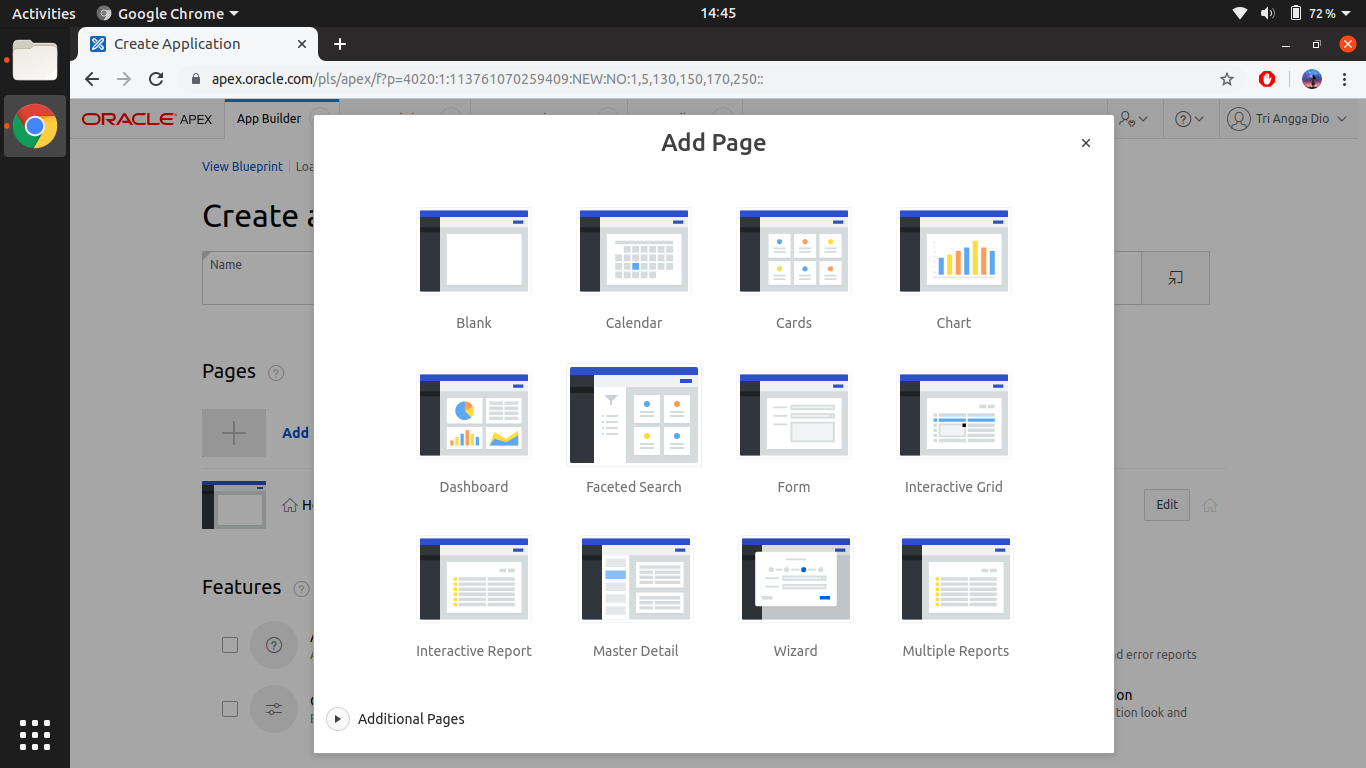
\includegraphics[scale=0.5]{figures/26.png}
    \caption{Add page}
    \label{fig:my_label}
\end{figure}
\newline
\item Setelah itu Create An application 
\newline
\begin{figure}[!htbp]
    \centering
    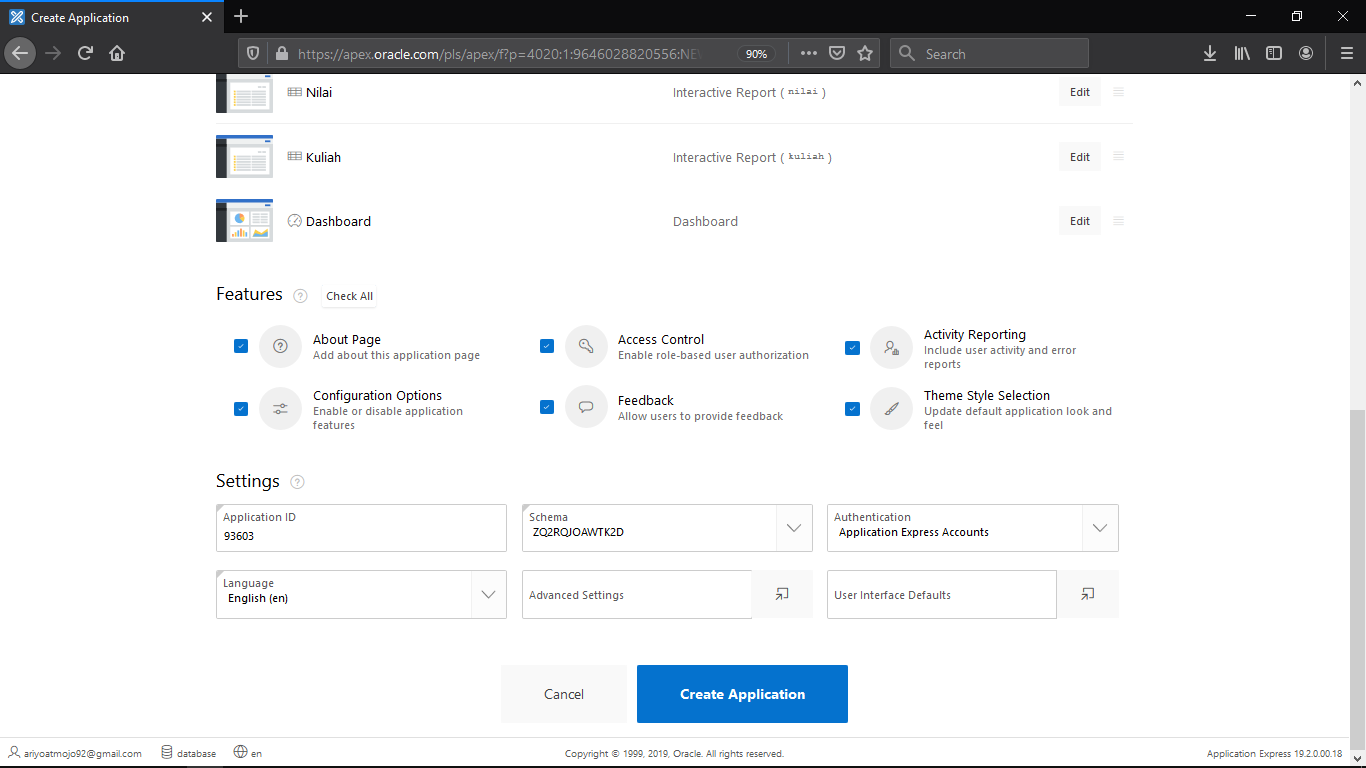
\includegraphics[scale=0.5]{figures/38.png}
    \caption{Create An Application}
    \label{fig:my_label}
\end{figure}
\newline
    \item  lalu klik check all
\newline
    \item  Maka selanjunya jalankan aplikasi dengan mengklik run application
\newline
\begin{figure}[!htbp]
    \centering
    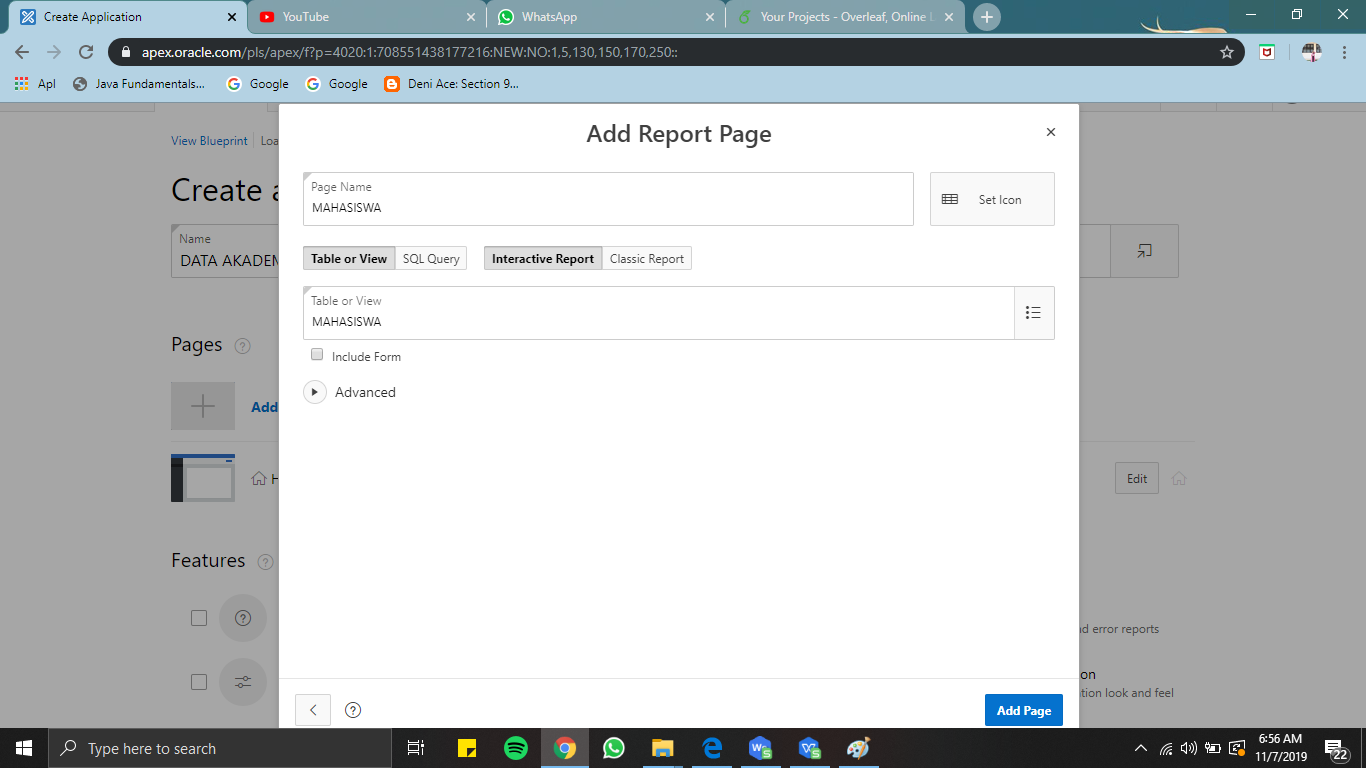
\includegraphics[scale=0.5]{figures/40.png}
    \caption{Run Application}
    \label{fig:my_label}
\end{figure}
\newline

\item Lalu masukkan email dan password untuk masuk ke aplikasi nya . 
\newline
\begin{figure}[!htbp]
    \centering
    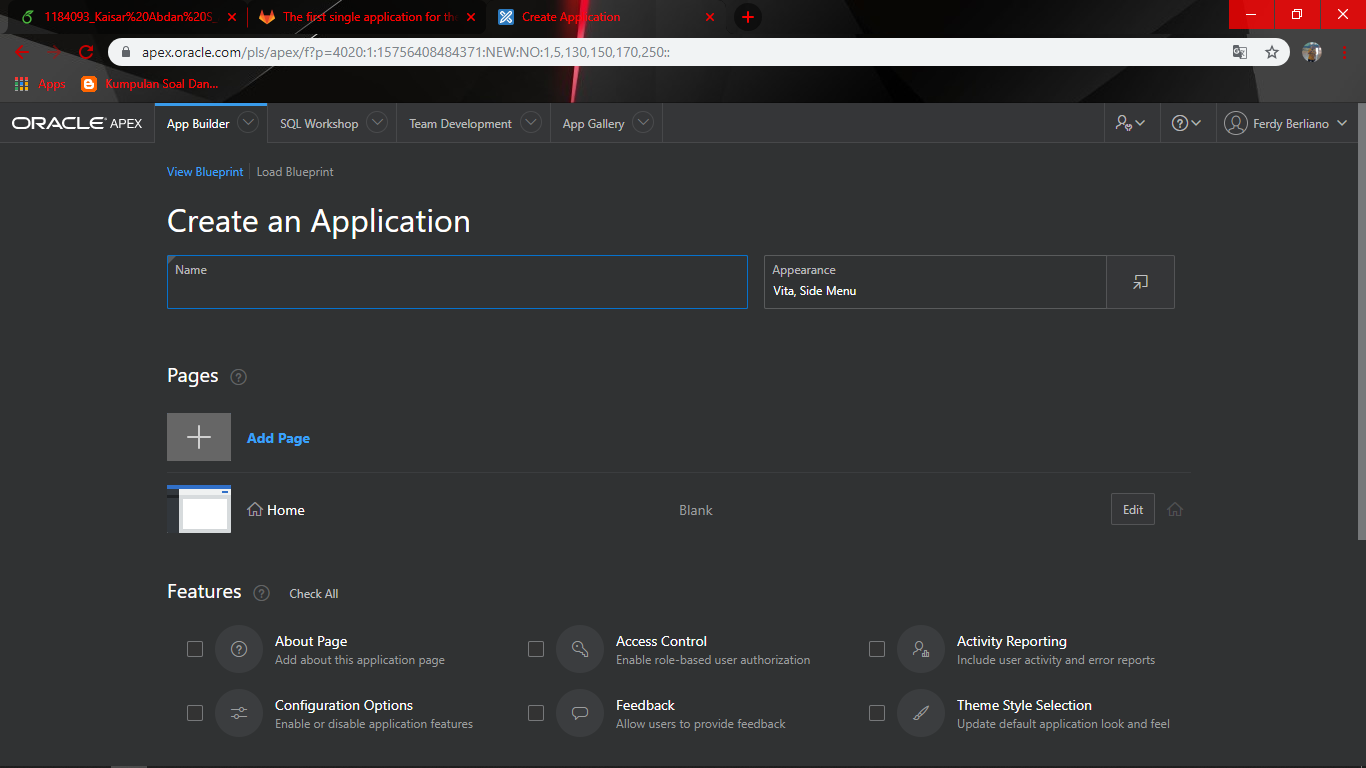
\includegraphics[scale=0.7]{figures/41.png}
    \caption{Sign in}
    \label{fig:my_label}
\end{figure}
\newline
    \item  Maka akan muncul aplikasi sistem sederhana akademik 
\newline
\begin{figure}[!htbp]
    \centering
    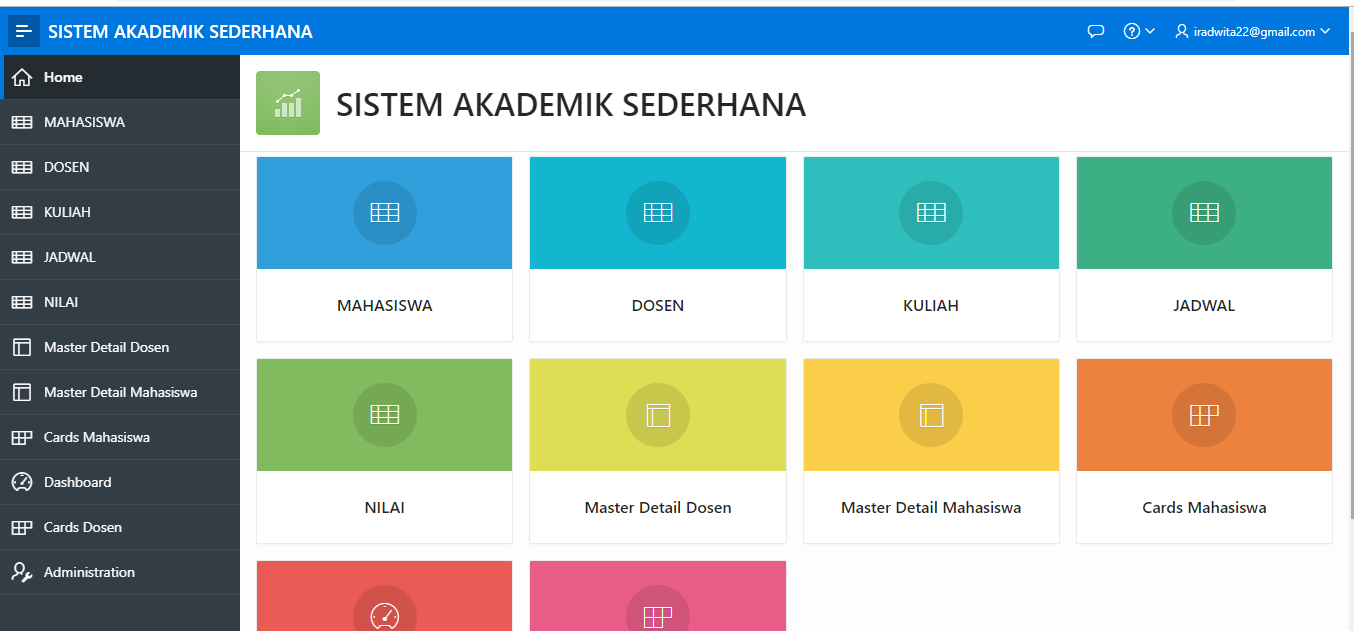
\includegraphics[scale=0.3]{figures/42.png}
    \caption{Aplikasi Sistem Akademik Sederhana}
    \label{fig:my_label}
\end{figure}
\newline
    \item  Aplikasi akademik selesai dibuat .
\end{enumerate}

link : https://apex.oracle.com/pls/apex/f?p=76816:LOGIN_DESKTOP:711761223598218:::::

Email : IRADWITA22@GMAIL.COM

Password :#Ira1234






\begin{enumerate}


\end{enumerate}

\chapter*{Link Oracle Express}
\section*{Data email password dan link oracle express} 


\item Email : jefriiimarbun@gmail.com
\item Password : jubilate300
\item https://apex.oracle.com/pls/apex/f?p=62374:1:20283547428623:::::

	
	
	

\chapter{Fungsi dan Kelas}
Tujuan pembelajaran pada pertemuan ketiga antara lain:
\begin{enumerate}
\item
Mengenal struktur fungsi di python dalam satu file dan cara pemanggilannya
\item
Mengerti cara membuat library fungsi dan melakukan import dan berbagai jenis import
\item
Mengerti struktur library kelas python dan cara pemakaiannya
\item
Mengatasi Error yang terjadi akibat pemakaian fungsi dan kelas
\item
Try Except
\end{enumerate}
Tugas dengan cara dikumpulkan dengan pull request ke github dengan menggunakan latex pada repo yang dibuat oleh asisten IRC. Kode program dipisah dalam folder src NPM.py yang berisi praktek dari masing-masing tugas file terpisah sesuai nomor yang kemudian dipanggil menggunakan input listing ke dalam file latex penjelasan atau nomor pengerjaan. Masing masing soal bernilai 5 dengan total nilai 100. Gunakan bahasa yang baku dan bebas plagiat dengan dibuktikan hasil scan plagiarisme. Serta hasil scrinsut dari komputer sendiri, dan kode hasil sendiri.

\section{Contoh Program}
\subsection{Fungsi}
Fungsi adalah satu blok program yang terdiri dari nama fungsi, input variabel dan variabel kembalian. Nama fungsi diawali dengan \textit{def} dan setelahnya tanda titik dua. Nama bisa sama dengan isi berbeda jika menggunakan huruf besar dan kecil atau sering disebut dengan \textit{case sensitive}. Input variabel bisa lebih dari satu dengan pemisah tanda koma. variabel kembalian pasti satu, bebas apakan itu jenis \textit{string}, \textit{integer}, \textit{list} atau \textit{dictionary}. Contoh dari fungsi sederhana bisa dilihat pada listing \ref{lst:fungsisederhana}. Dimana hasil akhir variabel c adalah 15.
\begin{lstlisting}[caption=Fungsi Sederhana,label={lst:fungsisederhana}]
def Penambahan(a,b):
	r = a + b
	return r
	
	
a=2
b=13
c = Penambahan(a,b)
\end{lstlisting}
sekarang kita pisah fungsi dengan pemakaian fungsi tersebut dalam file terpisah. Kita buat file bernama \textit{kalkulator.py} yang berisi semua fungsi penambahan, pengurangan, perkalian dan pembagian seperti terlihat pada listing \ref{lst:kalkulatorlib}. Sehingga satu file yang hanya berisi semua fungsi ini kita namakan \textit{paket} atau \textit{library}.
\begin{lstlisting}[caption=Library atau Paket kalkulator,label={lst:kalkulatorlib}]
def Penambahan(a,b):
	r = a + b
	return r
def Pengurangan(a,b):
	r = a - b
	return r
def Perkalian(a,b):
	r = a * b
	return r
def Pembagian(a,b):
	r = a / b
	return r
\end{lstlisting}
	Dan satu file yang memakai fungsi tersebut dengan nama file \textit{main.py}. Karena file kalkulator.py merupakan sebuah library maka kita panggil dulu dengan menggunakan perintah \textit{import}. Harus diingat file \textit{kalkulator.py} harus satu folder dengan \textit{main.py} yang berisi seperti listing\ref{lst:pakaikalkulator}.
\begin{lstlisting}[caption=Cara penggunaan library kalkulator,label={lst:pakaikalkulator}]
import kalkulator

a=100
b=50
hasil1=kalkulator.Penambahan(a,b)
hasil2=kalkulator.Pengurangan(a,b)
hasil3=kalkulator.Perkalian(a,b)
hasil4=kalkulator.Pembagian(a,b)
\end{lstlisting}
Maka kita bisa lihat hasilnya pada variabel hasil1, hasil2, hasil3, hasil4. Pada variabel exporer di spyder.

\subsection{Kelas}
Dasarnya dari kelas adalah pemrograman berbasis objek. Maka kita harus ingat, ada kelas ada objek ada atribut ada method. Fungsi kalkulator kita ubah menjadi kelas Ngitung.py menjadi seperti pada listing \ref{lst:kelasngitung}.
\begin{lstlisting}[caption=Kelas library kalkulator,label={lst:kelasngitung}]
class Ngitung:
  def __init__(self, a, b):
    self.a = a
    self.b = b
  def Penambahan(self):
    r = self.a + self.b
    return r
  def Pengurangan(self):
    r = self.a - self.b
    return r
  def Perkalian(self):
    r = self.a * self.b
    return r
  def Pembagian(self):
    r = self.a / self.b
    return r
\end{lstlisting}
Dana pada file main.py untuk menggunakan kelas maka bedanya adalah penambahan variabel yang menjadi objek instansiasi dari kelas seperti terlihat pada listing \ref{lst:instanngitung}.
\begin{lstlisting}[caption=Cara penggunaan kelas library kalkulator,label={lst:instanngitung}]
import ngitung

a=100
b=50

hitung = ngitung.Ngitung(a,b)

hasil1=hitung.Penambahan()
hasil2=hitung.Pengurangan()
hasil3=hitung.Perkalian()
hasil4=hitung.Pembagian()
\end{lstlisting}



\section{Pemahanan Teori}
Kerjakan soal berikut ini, masing masing bernilai 5. 
Praktek teori penunjang yang dikerjakan :
\begin{enumerate}
\item
Apa itu fungsi, inputan fingsi dan kembalian fungsi dengan contoh kode program lainnya.
\item
Apa itu paket dan cara pemanggilan paket atau library dengan contoh kode program lainnya.
\item
Jelaskan Apa itu kelas, apa itu objek, apa itu atribut, apa itu method dan contoh kode program lainnya masing-masing.
\item
Jelaskan cara pemanggikan library kelas dari instansiasi dan pemakaiannya dengan contoh program lainnya.
\item
Jelaskan dengan contoh pemakaian paket dengan perintah \textit{from kalkulator import Penambahan} disertai dengan contoh kode lainnya.
\item
Jelaskan dengan contoh kodenya, pemakaian paket fungsi apabila file library ada di dalam folder.
\item
Jelaskan dengan contoh kodenya, pemakaian paket kelas apabila file library ada di dalam folder.
\end{enumerate}

\section{Ketrampilan Pemrograman}
Kerjakan soal berikut ini, masing masing bernilai 5. Pada pertemuan sebelumnya tentang pembuatan program di python, sekarang cobalah untuk membuat nya dalam bentuk fungsi dan kelas dengan ketentuan:
\begin{enumerate}
\item
Buatlah fungsi dengan inputan variabel NPM, dan melakukan print luaran huruf yang dirangkai dari tanda bintang, pagar atau plus dari NPM kita.
Tanda bintang untuk NPM mod 3=0, tanda pagar untuk NPM mod 3 =1, tanda plus untuk NPM mod3=2.
Contoh Output : 
\begin{verbatim}
*****    *** ******     *****    ****
*******  *** ***  **    *** **  *****
***  ******* ******     ***  **** ***
***    ***** ***        ***       ***
***     **** ***        ***       ***
\end{verbatim}
NPM sesuai dengan nomor NPM nya.
\item
Buatlah fungsi dengan inputan variabel berupa NPM. kemudian dengan menggunakan perulangan mengeluarkan print output sebanyak dua dijit belakang NPM, 
contoh NPM : 113040087 maka akan ada output sebanyak 87 dengan tulisan `Hallo, 113040087 apa kabar?'
\begin{verbatim}
Output : 
Halo, 113040087 apa kabar? 
Halo, 113040087 apa kabar?
Halo, 113040087 apa kabar?
Halo, 113040087 apa kabar?
Halo, 113040087 apa kabar?
Halo, 113040087 apa kabar?
Halo, 113040087 apa kabar?
Halo, 113040087 apa kabar?
.....87 kali...
\end{verbatim}
\item
Buatlah fungsi dengan dengan input variabel string bernama \textbf{NPM} dan beri luaran output dengan perulangan berupa tiga karakter belakang dari NPM sebanyak penjumlahan tiga dijit tersebut. Penjumlahan dilakukan dengan menggunakan operator aritmatika dan fungsi int() atau str().
\begin{verbatim}
Output : Halo, Nama apa kabar? 
Halo, 087 apa kabar?
Halo, 087 apa kabar?
Halo, 087 apa kabar?
Halo, 087 apa kabar?
Halo, 087 apa kabar?
Halo, 087 apa kabar?
Halo, 087 apa kabar?
........15 kali(0+8+7).........
\end{verbatim}
\item
Buatlah fungsi hello word dengan input variabel string bernama \textbf{NPM} dan beri luaran output berupa digit ketiga dari belakang dari variabel NPM menggunakan akses langsung manipulasi string pada baris ketiga dari variabel NPM.
\begin{verbatim}
Input : 113040087
Output :
Halo, 0 apa kabar?
\end{verbatim}
\item

\label{digitvar2}
(wajib menggunakan perulangan dan atau kondisi) buat fungsi program dengan input variabel NPM dan melakukan print nomor npm satu persatu kebawah.
Contoh untuk NPM : 113040087 maka,
\begin{verbatim}
1
1
3
0
4
0
0
8
7
\end{verbatim}
\item
Buatlah fungsi dengan inputan variabel NPM, didalamnya melakukan penjumlahan dari seluruh dijit NPM tersebut, wajib menggunakan perulangan dan atau kondisi.
\item 
Buatlah fungsi dengan inputan variabel NPM, didalamnya melakukan melakukan perkalian dari seluruh dijit NPM tersebut, wajib menggunakan perulangan dan atau kondisi.
\item
Buatlah fungsi dengan inputan variabel NPM, Lakukan print NPM anda tapi hanya dijit genap saja. wajib menggunakan perulangan dan atau kondisi. Contoh jika NPM :113040087.
\begin{verbatim}
48
\end{verbatim}
\item
Buatlah fungsi dengan inputan variabel NPM, Lakukan print NPM anda tapi hanya dijit ganjil saja. wajib menggunakan perulangan dan atau kondisi. Contoh jika NPM :113040087.
\begin{verbatim}
1137
\end{verbatim}
\item 
Buatlah fungsi dengan inputan variabel NPM, Lakukan print NPM anda tapi hanya dijit yang termasuk bilangan prima saja. wajib menggunakan perulangan dan atau kondisi. Contoh jika NPM :113040087.
\begin{verbatim}
37
\end{verbatim}
\item
Buatlah satu library yang berisi fungsi-fungsi dari nomor diatas dengan nama file 3lib.py dan berikan contoh cara pemanggilannya pada file main.py.
\item
Buatlah satu library class dengan nama file kelas3lib.py yang merupakan modifikasi dari fungsi-fungsi nomor diatas dan berikan contoh cara pemanggilannya  pada file main.py.
\end{enumerate}


\section{Ketrampilan Penanganan Error}
Kerjakan soal berikut ini, masing masing bernilai 5. Bagian Penanganan error dari script python.
\begin{enumerate}
\item
Tuliskan peringatan error yang didapat dari mengerjakan praktek ketiga ini, dan jelaskan cara penanganan error tersebut.
dan Buatlah satu fungsi yang menggunakan gunakan try except untuk menanggulangi error yang kemungkinan akan terjadi.
\end{enumerate}


\chapter{PENYUSUNAN LAPORAN}
\section{Tujuan}
Untuk	 melaporkan	 jalannya	 pekerjan	 Proyek	 serta	 hasil	 yang	 diperoleh,	 mahasiswa	diwajibkan	menyusun	laporan	pekerjaan	Proyek.

\section{Ketentuan Penyusunan Laporan}
\subsection{Format Laporan}
Laporan	Proyek	hendaknya	berisi	:

\begin{enumerate}
\item \textbf{ Bagian Awal}
	\begin{itemize}
		\item Lembar	Muka	
		\item Lembar Pengesahan
		\item Surat	Pernyataan	Tidak	Melakukan	Plagiarisme
	 \item Abstrak	(dalam	Bahasa	Indonesia)
	 \item Abstract(dalam	Bahasa	Inggris)
	 \item Kata	Pengantar
	 \item Daftar	Isi	termasuk	:
 \begin{enumerate}[label=(\alph*)]
 
	\item Daftar	Gambar
	\item Daftar	Tabel
	\item Daftar	Simbol
	\item Daftar	Singkatan	
	\item Daftar	Lampiran
 \end{enumerate}
 \end{itemize}
 
\item \textbf{Bagian Isi}
 	\par \textbf{BAB	I PENDAHULUAN}
 	
 	\begin{enumerate} [label=1.\arabic*]
 	\item \textbf{ Latar	Belakang} \par 
Berisi	ulasan	ringkas	mengenai	keadaan/kondisi	yang	ada	dan	
kekurangan	 dari	 sistem	 yang	 diamati	 sehingga	 muncul	 topik	
yang	diambil.

\item \textbf{ Identifikasi	Masalah} \par 
Berisi	 berbagai	 masalah	 yang	 sudah	 dikenali	 dan	 	 akan diberikan	 solusinya	 melalui	 fungsi	 dari	 sistem/aplikasi/alat	yang	akan	dibuat.

\item \textbf{Tujuan} \par
Berisi	tujuan	untuk	apa	sistem/aplikasi/alat	itu	dibuat.

\item \textbf{ Ruang	Lingkup	} \par
Berisi	batasan-batasan	proyek	atau	cakupan	aplikasi	yang	akan	
dibangun.

\item \textbf{ Sistematika	Penulisan} \par
Menjelaskan	isi	yang	ada	di	laporan	proyek.\\
 
 	\end{enumerate}
 	
 \par \textbf{BAB II LANDASAN TEORI} \par 
 
 	Uraian	 \textbf{tentang	 teori yang	 mendukung} Objek	 PROYEK 2.	 \textbf{Harus	jelas	 sumber	 rujukannya	 dari	 mana}. Sumber	 yang	 baik	 adalah	jurnal	 ilmiah,	 artikel	 ilmiah,	 buku,	 dll.	 \textit{\textbf{Disarankan	 untuk	 tidak	mengambil	sumber	seperti	WebBlog,	Wikipedia,	dll.}} \\
 	
 	\par \textbf{BAB III ANALISIS DAN PERANCANGAN} \par 
 	\textit{\textbf{Analisis}} : \par 
 	Proses	 untuk	 menentukan	 bentuk	 dari	 kebutuhan	
sistem/aplikasi/alat	 baik	 berupa	 kebutuhan	 pada	 saat	membangun	
maupun	pada	saat	Implementasi.

	\textit{\textbf{Perancangan}}: \par 
	Penjelasan	 perancangan	 	 sistem/aplikasi/alat	 	 yang	 akan	 dibuat	terdiri	dari	perancangan	alir	program \textit{\textbf{(Flow	Chart)}}	, algoritma,	data,	maupun	perancangan	input/output	sistem/aplikasi/alat.		
 	
	
	\begin{enumerate} [label=3.\arabic*]
		\item Analisis
			\begin{enumerate} [label=3.1.\arabic*]
				\item Analisis	Sistem	yang	Sedang	Berjalan
					\begin{enumerate} [label=3.1.1.\arabic*]
						\item Analisis	Prosedur/ \textit{Flow	Map} yang								  berjalan
						\item Analisis	Dokumen	yang digunakan
					\end{enumerate}
				\item Analisis	Sistem	yang	akan	Dibangun
					\begin{enumerate} [label=3.1.2.\arabic*]
						\item Analisis	Kebutuhan	Aplikasi
						\item Analisis	Kebutuhan	Perangkat	lunak									  dan	Perangkat Keras
					\end{enumerate}
			\end{enumerate}
			
			
		\item Perancangan \textit{\textbf{(Jika	menggunakan	procedural 					  atau DFD)}}
			\begin{enumerate} [label=3.2.\arabic*]
				\item \textit{Context	Diagram}
				\item \textit {Data	Flow	Diagram} (disertai	tabel									  spesifikasi	Proses)
				\item Kamus	Alir	Data \textit{(Data Dictionary)}
				\item 	Perancangan	 \textit{Database (Sesuaikan	Format							Penulisannya)}
					\begin{enumerate} [label=3.2.4.\arabic*]
						\item \textit{Conceptual	Data	Model}
						\item \textit{Physical	Data	Model}
						\item \textit{Kamus	Data	Tabel (Database)}	
					\end{enumerate}
				\item Struktur Menu
				\item Perancangan Antarmuka
			\end{enumerate}
			
	\end{enumerate}
			
			\begin{enumerate} [label=3.2]
				\item Perancangan \textit{\textbf{(Jika	menggunakan 							  	Object	Oriented UML)}}
			\end{enumerate}
				\begin{enumerate} [label=3.2.\arabic*]
				\item \textit{Use	Case	Diagram}
				\item \textit{Class	Diagram}
				\item \textit{Interaction	Diagram}
				\item \textit{Sequence	Diagram}
				\item \textit{Collaboration	Diagram}
				\item \textit{Activity	Diagram}
				\item \textit{Statechart	Diagram}
				\item \textit{Componen	Diagram}
				\item \textit{Deployment	Diagram}
				\item \textit{Objek	Diagram}
				\item Perancangan \textit{Database (Sesuaikan	Format							  Penulisannya)}
						\begin{enumerate}[label=(\alph*)]
							\item \textit{Conceptual Data Model	(CDM)}
							\item \textit{Physical	Data Model (PDM)}
						\end{enumerate}
				\item Struktur	Menu
				\item Perancangan	Antarmuka
				\end{enumerate} 
				
	\par \textbf{BAB IV IMPLEMENTASI DAN PENGUJIAN} \par 
	\textbf{Implementasi} : \par 
	adalah	sistem/aplikasi/alat	yang	dibuat	dengan	merinci	komponenkomponen	 pendukung	 berupa	 program,	 Lingkungan	 Implementasi, Tampilan	Antarmuka,	Petunjuk	Pemakaian,	Petunjuk	Instalasi.
	
	\textbf{Pengujian} : \par 
	Adalah	 Cara	 untuk	 mengetahui	 apakah	 sistem/aplikasi/alat	 yang dibuat	sesuai	dengan	rancangan	dan	menuliskan	hasil	ujinya.
\textit{Jika	 anda	 membuat	 analisis	 sistem/aplikasi,	 maka	 harus	 seperti berikut:}
	
	\begin{enumerate} [label=4.\arabic*]
		\item Lingkungan	Implementasi \par 	
		Berisi	 perangkat	 lunak	 dan	 perangkat	 keras	 apa	 saja yang	digunakan	 sewaktu	 perancangan	 aplikasi	 berupa	 sistem	operasi,	database,	prosesor,	memory,	space	harddisk	dan	lain-lain	sesuai	dengan	kebutuhan serta	perangkat	pendukungnya.
		
		\item Pembahasan	Hasil	Implementasi \par 
		Berisi	 uraian	 hasil	 implementasi	 sistem	 yang	 disesuaikan	dengan	 tujuan	 pembuatan	 sistem.	 Jelaskan bahwa	 masalah	 yang	teridentifikasi	 pada	 identifikasi	 masalah yang berada	 di	 bab	 1	 telah	terseleseaikan, dan	 tujuan	 dari	 pelaksanaan	 proyek	telah tercapai. Penjelasan	dibantu	dengan	Tampilan	Antarmuka	aplikasi.
		
		\item Pengujian	dan	hasil	Pengujian \par 
		Berisi	identifikasi	 pengujian,	 rencana	 pengujian,	 deskripsi dan hasil	uji.	Metoda	yang	digunakan	misalnya \textit{white	box testing} dan \textit{	black	box	testing}
		
	\end{enumerate}	 
	
	
	
	\par \textbf{BAB V KESIMPULAN	DAN	SARAN} \par 
	
	\begin{enumerate} [label=5.\arabic*]
		\item \textbf{Kesimpulan} : \par 
				berisi	pencapaian	tujuan	dari	sistem/aplikasi/alat	                yang	dibuat.
		\item \textbf{Saran} : \par 
				berisi	hal-hal	atau	tujuan	dari	pembuatan	sistem/aplikasi/alat	yang dirasa	belum	sempurna	atau	 tidak	 tercapai.	Saran	juga	bisa	berupa	kondisi	 implementasi	 yang	 optimal	 bagi	 sistem/aplikasi/alat	 yang dibuat.
	\end{enumerate}
			
			
\item Bagian Akhir
 \begin{itemize}
 	\item Daftar	Pustaka		(Lampiran	8)
 	\item Lampiran
 	\item Tabel-tabel
 \end{itemize} 
 		 	
\end{enumerate}

\section{Ukuran	Kertas	dan	Ukuran	Huruf}

\begin{itemize}
	\item Penulisan	 dan	 ejaan	 menggunakan	 ketentuan	 bahasa	 Indonesia	 yang	 baik	 dan	
benar;
	\item Penulisan	diketik	dengan	komputer,	dengan	ketentuan	:
		\begin{enumerate}
			\item Jarak	1,5 spasi ;
			\item Lebar	sembir	kiri	4	cm ;
			\item Lebar	sembir	kanan	2,5	cm ;
			\item Lebar	sembir	atas	3	cm ;
			\item Lebar	sembir	bawah	3	cm ;
			\item Ukuran	Font	adalah	\textit{Times	New	Roman} 12	Kecuali	untuk	judul	bab	menggunakan	\textit{Times New Roman} dengan	ukuran	14.
		\end{enumerate}
		
	\item Ukuran	buku	adalah	A4	(21	x	29,7	Cm),	dengan	berat	kertas	80	gram;
	
	\item Sampul	depan	adalah	mika/softcover mika,	dengan	ketentuan	seperti	ini	:
		\begin{enumerate}
			\item Proposal	Proyek   \qquad \qquad \enspace : Mika Transparan .
			\item Buku Laporan Proyek \qquad : \textit{Softcover} Merah Omega 17.
		\end{enumerate}
		
		
\section{Ketentuan	Khusus}
	\begin{enumerate}
		\item \textbf{Abstrak} : Jarak	 1	 spasi,	 maksimal	 1	 halaman,	 font	 12,	 italic,	 maksimum	 200	 kata.
Hanya	1	paragraf. Kata	kunci	minimal	5.

		\item Penomoran	 tabel	 dilakukan	 dengan	 menyebutkan	 nomor	 bab,	 diikuti	 nomor	 urut	tabelnya	pada	bab	tersebut,	misalnya	Tabel	3.7,	artinya	tabel	nomor 7	di	bab	3.	Judul	
tabel	 diletakkan	 di	 atas	 tabel,	 penulisannya	 dengan	 huruf	 kapital	 di	 awal	 kata.	 Bila	tabel	 lebih	 panjang	 dari	 halaman,	 maka	 sambungan	 tabel	 pada	 halaman	 berikutnya	
diberi	judul	dengan	tulisan	: \textbf{(Lanjutan)}
		\item Tulisan	di	dalam	tabel	Jarak	1 spasi,	ukuran	huruf kurang	atau	sama	dengan \textit{font} 10 ( $\leq \textit{font}  10$). 	Judul	tabel	disimpan diatas	table	tanpa	jarak	spasi.
		
		\item Penomoran	 gambar	 dilakukan	 dengan	menyebutkan	 nomor	 bab,	 diikuti	 nomor	 urut	gambarnya	pada	bab	tersebut,	misalnya		Gambar	2.5,	artinya	gambar	nomor	5	di	bab	
2.			 Judul	gambar	diletakkan	di	bawah	gambar,	penulisannya	dengan	huruf	kapital	di	awal	kata.

		\item Penomoran	 halaman	 dimulai	 dari	 nomor	 1	 untuk	 tiap	 bab	 atau	 lampiran,	 dengan	
ketentuan	sebagai	berikut:	\\
			Penomoran	 dari	 bab	 1	 sampai	 bab	 5	 dimulai	 dari	 halaman	 1	 sampai	 selanjutnya	sekuensial	tanpa	menggunakan	bab	contoh	;	pada	awal	bab	2,	jika	bab	1	sebanyak	10	halaman,	maka	bab	2	dimulai	dengan	halaman	11	dst. .
			
		\item Penomoran	 halaman	 judul,	 buku	 laporan,	 halaman	 	 persetujuan,	 Daftar	 Isi,	 Daftar	Tabel,	dan	Daftar		Gambar	menggunakan	i,		ii,		iii,	…..	(angka	romawi	kecil).
		
		\item Setelah	Buku	laporan	 ditandatangani	 oleh	 pembimbing	 dan	 penguji	 seminar/sidang,	
maka	harus	di	buatkan	Jurnal	dengan	jumlah	halaman	maksimum	6	halaman.

		\item \textit{Softcopy} dari	jurnal, \textit{software} dan	laporan	disimpan	dalam	sebuah	CD	dan	disertakan	
ke	dalam	laporan di	beri	judul	serta	penulis	di	label	CD	nya.

	\end{enumerate}
\end{itemize}

\section{Status	Buku}
\begin{enumerate}
	\item Status Buku \par 
		Buku	 yang	 memenuhi	 persyaratan	 untuk	 sidang Proyek	 adalah	 buku	 yang	 telah	
selesai	 100 \%.	 Penjilidan	 buku	 sebelum	 sidang menggunakan	 penjepit	 dan	 sampul	plastik	mika	warna	Transparan;

	\item Setelah	Sidang \par 
		Buku	 yang	 memenuhi	 persyaratan	 untuk	 keluarnya	 nilai	 adalah	 buku	 yang	 telah	selesai	 100 \%	 (telah	 diperbaiki,	 jika	 ada	 tugas	 perbaikan).Penjilidan	 	 buku	 setelah	sidang dan	 setelah	 melalui	 perbaikan	 adalah	 jilid	 punggung	 disertai	 halaman	pembatas	bab	warna	merah	seperti	pita	pembatas	warna	merah.	
		
\end{enumerate}

\section{Distribusi	Buku}
Jumlah	 salinan	 laporan	 Proyek	 untuk	 keperluan	 sidang Proyek	 adalah	 3	 \textit{copy},	 dengan	distribusi	sebagai	berikut	:

\begin{enumerate}
	\item Pembimbing/Ketua	Penguji \quad (1 copy)
	\item Anggota	Penguji \qquad \qquad \qquad(1 copy)
	\item Mahasiswa \qquad \qquad \qquad \enspace \quad \quad(1 copy)
\end{enumerate}

Jumlah	salinan	buku	laporan	Proyek		adalah	4	 (empat) \textit{	 copy},	dengan	distribusi	sebagai	berikut	:

\begin{table}[H]
\label{tab:my-table}
\begin{tabular}{lll}
1 & Pembimbing & (1 CD) \\ \\
2 & Perpustakaan	Politeknik	Pos	Indonesia & (1 Buku dan CD ) \\ \\
3 & Mahasiswa & (1 Buku) \\ \\
4 & \multicolumn{2}{l}{\begin{tabular}[c]{@{}l@{}}Prodi	(1	 CD yang	 berisi	 jurnal,	 aplikasi	 dan	 laporan) dan	 hardcopy	 jurnal	 1	 buah	\\ tanpa	di	jilid.\end{tabular}}
\end{tabular}
\end{table}

\chapter{Komunikasi Perangkat Keras}

Tujuan pembelajaran pada pertemuan kelima antara lain:
\begin{enumerate}
\item
Mengenal komunikasi data serial
\item
Mengerti cara memakai library PySerial
\item
Mengerti cara instalasi driver dan menemukan BaudRate dan Nomor Port
\item
Mengatasi Error yang terjadi akibat pemakaian library csv dan pandas
\item
Try Except
\end{enumerate}
Tugas dengan cara dikumpulkan dengan pull request ke github dengan menggunakan latex pada repo yang dibuat oleh asisten IRC. Kode program dipisah dalam folder src NPM.py yang berisi praktek dari masing-masing tugas file terpisah sesuai nomor yang kemudian dipanggil menggunakan input listing ke dalam file latex penjelasan atau nomor pengerjaan. Masing masing soal bernilai 5 dengan total nilai 100. Gunakan bahasa yang baku dan bebas plagiat dengan dibuktikan hasil scan plagiarisme. Serta hasil scrinsut dari komputer sendiri, dan kode hasil sendiri. Pengerjaan menggunakan latex dan harus menyertakan file pdf hasil compile pdflatex, jika tidak diskon 50\%.


\section{Pemahaman Teori}
Kerjakan soal berikut ini, masing masing bernilai 5. Untuk hari pertama.
Praktek teori penunjang yang dikerjakan dengan deadline rabu jam 4 pagi:
\begin{enumerate}
\item
Apa itu fungsi device manager di windows dan folder /dev di linux
\item
Jelaskan langkah-langkah instalasi driver dari arduino
\item
Jelaskan bagaimana cara membaca baudrate dan port dari komputer yang sudah terinstall driver
\item
Jelaskan sejarah library pyserial
\item
Jelaskan fungsi-fungsi apa saja yang dipakai dari library pyserial
\item
Jelaskan kenapa butuh perulangan dalam tidak butuh perulangan dalam membaca serial
\item
Jelaskan bagaimana cara membuat fungsi yang mengunakan pyserial
\end{enumerate}

\section{Ketrampilan Pemrograman}
Kerjakan soal berikut ini, masing masing bernilai 10 untuk hari kamis jam 4 pagi. Soalnya adalah:

\begin{enumerate}
\item
Buatlah fungsi (file terpisah/library dengan nama NPM\_realtime.py) untuk mendapatkan data langsung dari arduino
\item
Buatlah fungsi (file terpisah/library dengan nama NPM\_save.py) untuk mendapatkan data langsung dari arduino dengan looping
\item
Buatlah fungsi (file terpisah/library dengan nama NPM\_realtime.py) untuk mendapatkan data dari arduino dan langsung ditulis kedalam file csv
\item
Buatlah fungsi (file terpisah/library dengan nama NPM\_csv.py) untuk membaca file csv hasil arduino dan mengembalikan ke fungsi
\end{enumerate}




\section{Ketrampilan Penanganan Error}
Kerjakan soal berikut ini, masing masing bernilai 5(hari kedua). Bagian Penanganan error dari script python.
\begin{enumerate}
\item
Tuliskan peringatan error yang didapat dari mengerjakan praktek ketiga ini, dan jelaskan cara penanganan error tersebut.
dan Buatlah satu fungsi yang menggunakan gunakan try except untuk menanggulangi error tersebut.
\end{enumerate}



\section{Presentasi Tugas}
Pada pertemuan ini, diadakan dua penilaiain yaitu penilaian untuk tugas mingguan seperti sebelumnya dengan nilai maksimal 100. Kemudian dalam satu minggu kedepan maksimal sebelum waktu mata kuliah pemrograman 3. Ada presentasi kematerian dengan nilai presentasi yang terpisah masing-masing 100. Jadi ada tiga komponen penilaiain pada pertemuan ini yaitu :
\begin{enumerate}
	\item tugas minggu hari ini dan besok (maks 100). pada chapter ini
	\item presentasi pyserial (maks 100). Mempraktekkan kode python dan menjelaskan cara kerjanya.
\end{enumerate}
Waktu presentasi pada jam kerja di IRC. Kriteria penilaian presentasi sangat sederhana, presenter akan ditanyai 20(10 pertanyaan program, 10 pertanyaan teori) pertanyaan tentang pemahamannya menggunakan python untuk kecerdasan buatan. jika presenter tidak bisa menjawab satu pertanyaan asisten maka nilai nol. Jika semua pertanyaan bisa dijawab maka nilai 100. Presentasi bisa diulang apabila gagal, sampai bisa mendapatkan nilai 100 dalam waktu satu minggu kedepan.





\chapter{Matplotlib}

Tujuan pembelajaran pada pertemuan kelima antara lain:
\begin{enumerate}
\item
Mengenal plot di python
\item
Mengerti cara memakai library Matplotlib
\item
Mengerti cara memplot berbagai macam jenis plot
\item
Mengatasi Error yang terjadi akibat pemakaian matplotlib
\item
Try Except
\end{enumerate}
Tugas dengan cara dikumpulkan dengan pull request ke github dengan menggunakan latex pada repo yang dibuat oleh asisten IRC. Kode program dipisah dalam folder src NPM.py yang berisi praktek dari masing-masing tugas file terpisah sesuai nomor yang kemudian dipanggil menggunakan input listing ke dalam file latex penjelasan atau nomor pengerjaan. Masing masing soal bernilai 5 dengan total nilai 100. Gunakan bahasa yang baku dan bebas plagiat dengan dibuktikan hasil scan plagiarisme. Serta hasil scrinsut dari komputer sendiri, dan kode hasil sendiri. Pengerjaan menggunakan latex dan harus menyertakan file pdf hasil compile pdflatex, jika tidak diskon 50\%.


\section{Pemahaman Teori}
Kerjakan soal berikut ini, masing masing bernilai 5. Untuk hari pertama.
Praktek teori penunjang yang dikerjakan dengan deadline hari pertama jam 4 pagi:
\begin{enumerate}
\item
Apa itu fungsi library matplotlib
\item
Jelaskan langkah-langkah membuat sumbu X dan Y di matplotlib
\item
Jelaskan bagaimana perbedaan fungsi dan cara pakai untuk berbagai jenis(bar,histogram,scatter,line dll) jenis plot di matplotlib
\item
Jelaskan bagaimana cara menggunakan legend dan label serta kaitannya dengan fungsi tersebut
\item
Jelaskan apa fungsi dari subplot di matplotlib, dan bagaimana cara kerja dari fungsi subplot, sertakan ilustrasi dan gambar sendiri dan apa parameternya jika ingin menggambar plot dengan 9 subplot di dalamnya
\item
Sebutkan semua parameter color yang bisa digunakan (contoh: m,c,r,k,... dkk)
\item
Jelaskan bagaimana cara kerja dari fungsi hist, sertakan ilustrasi dan gambar sendiri
\item
Jelaskan lebih mendalam tentang parameter dari fungsi pie diantaranya labels, colors, startangle, shadow, explode, autopct
\end{enumerate}

\section{Ketrampilan Pemrograman}
Kerjakan soal berikut ini, masing masing bernilai 10 untuk hari kedua jam 4 pagi. Soalnya adalah:

\begin{enumerate}
\item
Buatlah librari fungsi (file terpisah/library dengan nama NPM\_bar.py) untuk plot dengan jumlah subplot adalah NPM mod 3 + 2
\item
Buatlah librari fungsi (file terpisah/library dengan nama NPM\_scatter.py) untuk plot dengan jumlah subplot NPM mod 3 + 2
\item
Buatlah librari fungsi (file terpisah/library dengan nama NPM\_pie.py) untuk plot dengan jumlah subplot NPM mod 3 + 2
\item
Buatlah librari fungsi (file terpisah/library dengan nama NPM\_plot.py) untuk plot dengan jumlah subplot NPM mod 3 + 2
\end{enumerate}




\section{Ketrampilan Penanganan Error}
Kerjakan soal berikut ini, masing masing bernilai 5(hari kedua). Bagian Penanganan error dari script python.
\begin{enumerate}
\item
Tuliskan peringatan error yang didapat dari mengerjakan praktek ketiga ini, dan jelaskan cara penanganan error tersebut.
dan Buatlah satu fungsi yang menggunakan gunakan try except untuk menanggulangi error tersebut.
\end{enumerate}



\section{Presentasi Tugas}
Pada pertemuan ini, diadakan dua penilaiain yaitu penilaian untuk tugas mingguan seperti sebelumnya dengan nilai maksimal 100. Kemudian dalam satu minggu kedepan maksimal sebelum waktu mata kuliah pemrograman 3. Ada presentasi kematerian dengan nilai presentasi yang terpisah masing-masing 100. Jadi ada tiga komponen penilaiain pada pertemuan ini yaitu :
\begin{enumerate}
	\item tugas minggu hari ini dan besok (maks 100). pada chapter ini
	\item presentasi matplotlib (maks 100). Mempraktekkan kode python dan menjelaskan cara kerjanya.
\end{enumerate}
Waktu presentasi pada jam kerja di IRC. Kriteria penilaian presentasi sangat sederhana, presenter akan ditanyai 20(10 pertanyaan program, 10 pertanyaan teori) pertanyaan tentang pemahamannya menggunakan python untuk kecerdasan buatan. jika presenter tidak bisa menjawab satu pertanyaan asisten maka nilai nol. Jika semua pertanyaan bisa dijawab maka nilai 100. Presentasi bisa diulang apabila gagal, sampai bisa mendapatkan nilai 100 dalam waktu satu minggu kedepan.





\chapter{Discussion}
Please tell more about conclusion and how to the next work of this study.
\chapter{CARA MERUJUK DAN MENULIS DAFTAR RUJUKAN (PUSTAKA)}
Pembuatan	daftar	pustaka \textbf{diwajibkan} menggunakan	 fitur	Reference	Bibiliography	di	Microsoft Office	sehingga	daftar	pustaka	tercipta	dengan	otomatis.\\
Cara	merujuk	daftar	pustaka	adalah	sebagai	berikut:
\begin{enumerate}
\item Daftar	Pustaka	disusun	menurut	urutan	kutipan	dan	diberi nomor	urut	mulai	dari	[1].
\item Judul	buku	tidak	boleh	disingkat.
\item Penyingkatan	kependekan	Jurnal	Ilmiah	harus	mengikuti	yang	telah	lazim	dilakukan.
\item Nama	keluarga	(nama	belakang)	ditulis	terlebih	dahulu,	diikuti	dengan	singkatan	nama	depan.
\item Semua	nama	pengarang	harus	ditulis	sesuai	dengan	urutannya	di		dalam	artikel	/	buku.
\end{enumerate}

\par Penjelasan	lebih	rinci	mengenai	cara	merujuk	dan	menulis	daftar	rujukan	dijelaskan	sebagai	
berikut

\section{Cara	Merujuk}
Perujukan	 dilakukan	 dengan	menggunakan	 nama	 	 akhir	 dan	 tahun	 di	 antara	 tanda	 kurung. Jika	ada	dua	penulis,	perujukan	dilakukan	dengan	cara	menyebut	nama	akhir	kedua	penulis	
tersebut.	Jika	penulisnya	lebih	dari	dua	orang,	penulis	rujukan	dilakukan	dengan	cara	penulis	nama	pertama	dari	penulis	 tersebut	diikuti	dengan \textit{dkk}. Jika	nama	penulis	 tidak	disebutkan,	yang	 dicantumkan	 dalam	 rujukan	 adalah	 nama	lembaga	 yang	menerbitkan,	 nama	 dokumen yang diterbitkan,	 atau	 nama	 koran.	 Untuk	 karya	 terjemahan,	 perujukan	 dilakukan	 dengan	cara	menyebutkan	nama	penulis	aslinya.	Rujukan	dari	dua	sumber	atau lebih	yang	ditulis	oleh penulis	yang	berbeda	dicantumkan	dalam	satu	tanda	kurung	dengan	titik	koma	sebagai	tanda	pemisahnya.

\section{Cara	Merujuk	Kutipan	Langsung}
\subsection{Kutipan	Kurang	dari	40	Kata}
Kutipan	 yang	 berisi	 kurang	 dari	 40	 kata	 ditulis	 di	 antara	 tanda	 kutip	 (“…”)	 sebagai	bagian	 yang	 terpadu	 dalam	 teks	 utama,	 dan	 diikuti	 nama	 penulis,	 tahun	 dan	 nomor	halaman.	 Nama	 penulis	 dapat	 ditulis	 secara	 terpadu	 dalam	 teks	 atau	 menjadi	 satu	dengan	tahun	dan	nomor	halaman	di	dalam	kurung.	Lihat	contoh	berikut. Nama	penulis disebut	dalam	teks	secara	terpadu \\
\\

\textbf{Contoh :}\\
Tersine	 (1994:	 28)	 menyatakan	 “tekanan	 pasar	 memaksa	 organisasi	 untuk	menghasilkan	produk	yang	lebih	beragam	dan	kemampuan	pengiriman	yang	lebih	baik” Nama	penulis	disebut	bersama	dengan	tahun	penerbitan	dan	nomor	halaman.
\\
\\

\textbf{Contoh :}\\
Hal	 tersebut	 berdasarkan	 pada	 pernyataan	 “tekanan	 pasar	memaksa	 organisasi	 untuk	menghasilkan	produk	yang	lebih	beragam	dan	kemampuan	pengiriman	yang	lebih	baik”	
(Tersine,	1994:28). \\
Jika	ada	tanda	kutip	dalam	kutipan,	digunakan	tanda kutip	tunggal	(‘…’).
\\
\\

\textbf{Contoh :}\\
Ini	sejalan	dengan	pernyataan	Bickelhaupt	yang	menyatakan	“Kontrak	asuransi	bersifat	pribadi	 (personal)	 dang	 ‘mengikuti’	 pribadi	 itu,	 bukan	 ‘mengikuti’	 harta	 yang	diasuransikan.”

\subsection{Kutipan	40	Kata	atau	Lebih}
Kutipan	yang	berisi	40	kata	atau	lebih	ditulis	tanpa	tanda	kutip	secara	terpisah	dari	teks	yang	mendahului,	 ditulis	 1,2	 cm	 dari	 garis	 tepi	 sebelah	 kiri	 kanan,	 dan	 diketik	 dengan	spasi	tunggal.	Nomor	halaman	juga	harus	ditulis.
\\
\\
\\
\textbf{Contoh :}\\
Harrington	 (1999	 :	 384)	 menarik	 kesimpulan	 sebagai	 berikut.“Making	 manufacturers	strictly	liable	for	all	consumer	losses	can	improve	safety	incentives	when	consumers	are	
uninformed	 about	 product	 risk,	 because	 strict	 liability	 gives	 manufacturers	 proper	incentives	 to	make	safe	products	and	induces	consumers	 to	purchase	 the	right	amount	of	risky	products.” \\
Jika	dalam	kutipan	 terdapat	paragraf	baru	lagi,	garis	barunya	dimulai	1,2	cm	dari	 tepi	
kiri	garis	teks	kutipan.

\subsection{Kutipan	yang	Sebagian	Dihilangkan}
Apabila	 dalam	 mengutip	 langsung	 ada	 kata-kata	 dalam	 kalimat	 yang	 dibuang,	 maka	kata-kata	yang	dibuang	diganti	dengan	tiga	titik. \\
\\

\textbf{Contoh :}\\
"Asuransi	konstruksi	menjamin	kerugian	akibat	kerusakan	fisik	pada	proyek	pekerjaan	teknik	sipil	…	disebabkan	kecelakaan	yang	terjadi	pada	masa	pembangunan.” \\

Apabila	ada	 kalimat	 yang	 	 dibuang,	maka	 kalimat	 yang	 dibuang	 diganti	 dengan	empat	titik.\\
\\

\textbf{Contoh :}\\
“Kerugian	 tidak	langsung	juga	 timbul	pada	bangunan	 yang	 tidak	memenuhi	 ketentuan	sehingga	harus	dilakukan penggantian	semua	atau	sebagian	bangunan	tersebut	….Maka	kerugian	 tak	 langsung	 ada	 berupa	 biaya	 membuka	 bagian	 yang	 tidak	 salah,	 nilai	 dari	bagian	yang	tidak	dirusakkan,	dan	perbedaan	nilai	bangunan	setelah	diperbaiki	dengan	nilai	bangunan	sebelumnya”	(Darmawi,	2000:144).

\subsection{Cara	Merujuk	Kutipan	Tidak	Langsung}
Kutipan	 yang	 disebutsecara	 tak	 langsung	 atau	 dikemukakan	 dengan	 bahasa	 penulis	 sendiri	ditulis	tanpa	tanda	kutip	dan	terpadu	dalam	teks.	Nama	penulis	bahan	kutipan	dapat	disebut	terpadu	 dalam	 teks,	 atau	 disebut	 dalam	 kurung	 bersama	 tahun	 penerbitannya.	 Jika	memungkinkan	nomor	halaman	disebut	terpadu	dalam	teks.
\\
\\
\textbf{Contoh :} \\
Skipper	 (1999:453)	 hanya	 melakukan	 peramalan	 permintaan	 dengan	 pendekatan	 regresi	linier.\\ Nama	penulis	disebut	dalam	kurung	bersama	tahun	penerbitannya.\\
\textbf{Contoh :}\\
Untuk	kasus	tersebut,	regresi	logistik	ternyata	memberikan	hasil	yang	lebih	baik	(Wolff,	2000	
:	144).

\subsection{Cara	Menulis	Daftar	Rujukan (Pustaka)}
Daftar	rujukan	merupakan	daftar	yang	berisi	buku,	makalah,	artikel,	atau	bahan	lainnya	yang	dikutip	 baik	 secara	 langsung	 maupun tidak	 langsung.	 Bahan-bahan	 yang	 dibaca	 akantetapi	tidak	dikutip	\textit{tidak	dicantumkan} 	dalam	daftar	rujukan,	sedangkan	semua	bahan	yang	dikutip	secara	langsung	ataupun	 tak	langsung	dalam	 teks \textit{harus} dicantumkan	dalam	daftar	 rujukan.	

Pada	 dasarnya,	 unsur	 yang	 ditulis	 dalam	 daftar	 rujukan	 secara	 berturut-turut	 	meliputi	 (1)	nama	penulis	ditulis	dengan	urutan	:	nama	akhir,	nama	awal,	dan	nama	 tengah,	 tanpa	gelar	akademik,	 (2)	 tahun	 penerbitan,	 (3)	judul,	 termasuk	 anak	judul	(\textit{subjudul}),(4)	 kota	 tempat	
penebitan,	 dan	 (5)	 nama	 penerbit.	 Unsur-unsur	 tersebut	 dapat	 bervariasi	 tergantung	 jenis	sumber	 pustakanya.	 Jika	 penulisnya	 lebih	 dari	 satu,	 cara	 penulisan	 namanya	 sama	 dengan	penulis	pertama	(Lampiran-8). \\

Nama	 penulis	 yang	 terdiri	 dari	 dua	 bagian	 ditulis	 dengan	 urutan:	 nama	 akhir	 diikuti	 koma,	nama	 awal	 (disingkat	 atau	 tidak	 disingkat	 tetapi	 harus	 konsisten	 dalam	 satu	 karya	ilmiah), diakhiri	dengan	 titik.	Apabila	sumber	yang	dirujuk	ditulis	oleh	lain,	semua	nama	penulisnya	harus	dicantumkan	dalam	daftar	rujukan.
\\
\\

\textbf{Rujukan dari Buku} \par


Tahun	 penerbitan	 ditulis	 setelah	 nama	 penulis,	 diakhiri	 dengan	 titik.	 Judul	 buku	 ditulis	dengan	 huruf	 miring,	 dengan	 huruf	 besar	 pada	 awal	 setiap	 kata,	 kecuali	 kata	
hubung.Tempat	penerbitan	dan	nama	penerbit	dipisahkan	dengan	titik	dua	(:). \\
\\
\textbf{Contoh :} \\
Magee,	J.	F.	\&	Boodman,	D.	M.	1967. \textit{Production	Planning	and	Inventory	Control.}	New	York: McGraw-Hill. \\
Jika	 ada	 beberapa	 buku	 yang	 dijadikan	 sumber	 ditulis	 oleh	 orang	 yang	 sama	 dan	diterbitkan	dalam	tahun	yang	sama	pula,	data	tahun	penerbitan	diikuti	oleh	lambang	a,	b,	
dan	 c,	 dan	 seterusnya	 yang	 urutunnya	 ditentukan	 secara	 kronologis	 atau	 berdasarkan	abjad	judul	buku-bukunya. \\
\\

\textbf{Contoh :} \\
Cummins,	J.	D.	1992a. \textit{Should	Automobile	Insurance	be	Compulsary?}	Cincinnati,	OH:	General	Publisher. \\
Cummins,	 J.	 D.	 1992b.	\textit{Should	 Automobile	 Insurance	 be	 Compulsary:	 The	 Second	Perspective}. Cincinnati,	OH:	General	Publisher.
\\
\\
\textbf{Rujukan dari Buku yang Berisi Kumpulan Artikel (Ada Editornya)}


Seperti	menulis	rujukan	dari	buku	ditambah	dengan	tulisan	(Ed.)	jika ada	satu	editor	dan	(Eds.)	jika	editornya	lebih	dari	satu,	di	antara	nama	penulis	dan	tahun	penerbitan. \\ \\

\textbf{Contoh :}
Park,	S.	\&	Browse,	R.	(Eds.).	1998. \textit{A	Text	on	Marine	Insurance}.	New	York:	Pogue. \\
Dijkstra	(Ed.).	1990. \textit{Logistics Management}. New	York:	The	Foundation	Presss.
\\
\\
\textbf{Rujukan dari Artikel dalam Buku Kumpulan Artikel (Ada Editornya)}


Nama	penulis	artikel	ditulis	di	depan	diikuti	dengan	tahun	penerbitan.	Judul	artikel	ditulis	tanpa	 cetak	 miring.	 Nama	 editor	 ditulis	 seperti	 menulis	 nama	 biasa,	 diberi	 keterangan	(Ed.)	bila	hanya	satu	editor,	dan	(Eds.)	bila	lebih	dari	satu	editor.	Judul	buku	kumpulannya	ditulis	dengan	huruf \textit{miring}, dan	nomor	halamannya	disebutkan	dalam	kurung.\\
\\
\textbf{Contoh :}\\
Hartley,	 J.T.,	Harker,	 J.O.	\&	Walsh,	D.A.	1980. Contemporary	 Issues	and	New	Directions	in	Adult	 Development	 of	 Learning	 and	Memory.	 Dalam	 L.W.	 Poon	 (Ed.) \textit{Aging	in	 the	 1980s:	Psychological	Issues}(hlm.	239-252).	Washington,	D.C.:	American	Psycological	Association.\\
 Hasan,	 M.Z.	 1990.	 Karakteristik	 Penelitian	 Kualitatif.	 Dalam	 Aminuddin	 (Ed.),\\ \textit{Pengembangan	Penelitian	Kualitatif	dalam	Bidang	Bahasa	dan	Sastra} (hlm.	12-25).	Malang:	HISKI	Komisariat	Malang	dan	YA3.
 \\
 \\
 \textbf{Rujukan dari Artikel dalam Jurnal}\\
 Nama	 penulis	 ditulis	 paling	 depan	 diikuti	 dengan	 tahun	 dan	 judul	 artikel	 yang	 ditulis	dengan	 cetak	 biasa,	 dan	 huruf	 besar	 pada	 setiap	 awal	 kata.	 Nama	 jurnal	 ditulis	 dengan	cetak	miring,	 dan	 huruf	awal	 dari	 setiap	 katanya	 ditulis	 dengan	 huruf	 besar	 kecuali	 kata	hubung.	Bagian	akhir	berturut-turut		ditulis		jurnal	tahun	keberapa,	nomor	berapa	(dalam	kurung),	dan	nomor	halaman	dari	artikel	tersebut.\\
\\
\textbf{Contoh :}\\
Wuhrer,	 J.	 1975.	Better	Group	 Corporate	Health	 Financing.	\textit{Journal	 of	Risk	 and	 Insurance}, 1(3):	47-50.
\\
\\
\textbf{Rujukan dari Artikel dalam Jurnal dari CD-ROM}
Nama	penulis	ditulis	paling	depan,	diikuti	oleh	 tanggal,	bulan,	dan	 tahun	(jika	ada).	 Judul	artikel	ditulis	dengan	cetak	biasa,	dan	huruf	besar	pada	setiap	huruf	awal	kata,	kecuali	kata	
sambung.	Nama	majalah	ditulis	dengan	huruf	kecil	kecuali	huruf	pertama setiap	kata,	dan	dicetak \textit{miring}. Nomor	halaman	disebut	pada	bagian	akhir.
\\
\\Suryana,	 1996.	 Optimalisasi	 Waktu	 Perjalanan	 dengan	 Translasi	 Nonlinier. \textit{Jurnal	Transportasi},	3(3):55-59.
\\
\\
\textbf{Rujukan dari Koran Tanpa Penulis}
\\
Nama		koran	ditulis	di	bagian	awal.	Tanggal,	bulan,	dan	tahun	ditulis	setelah	nama	koran,	
kemudian	judul	ditulis	dengan	huruf	besar-kecil	dicetak	miring	dan	diikuti	dengan	nomor	halaman.
\\
\\
\textbf{Contoh :}
Suara	Pembaruan.	26	Juni,	1998. \textit{Asuransi	Perjalanan	Wisata},	5.	
\\
\\
\textbf{Rujukan dari Lembaga yang Ditulis Atas Nama Lembaga Tersebut}
\\
Nama	 lembaga	 penanggung	 jawab	 langsung	 ditulis	 di	 depan,	 diikuti	 dengan	 tahun,	 judul	karangan	 yang	 dicetak	 miring,	 nama	 tempat	 penerbitan,	 dan	 nama	 lembaga	 yang	bertanggung	jawab	atas	penerbitan	karangan	tersebut.
\\
\\
\textbf{Contoh :}
\\
Dewan	Asuransi	Indonesia.	1989. \textit{Perkembangan	Bisnis	Asuransi	di	Indonesia	Periode}	1975-1985.	Jakarta:	Dewan	Asuransi	Indonesia.
\\
\\
\textbf{Rujukan Berupa Karya Terjemahan}\\
Nama	 penulis	asli	 ditulis	 di	 depan,	 diikuti	 tahun	 penerbitan	 karya	asli,	judul	 terjemahan,	nama	 penerjemah,	 tahun	 terjemahan,	 nama	 tempat	 penerbitan	 dan	 nama penerbit	terjemahan,.	 Apabila	 tahun	 penerbitan	 buku	 asli	 tidak	 dicantumkan,	 ditulis	 dengan	 kata \textit{Tanpa	tahun}.
\\
\\
\textbf{Contoh :} \\
Zaelani,	 G.	 1989. \textit{Suatu	 Tinjauan	 tentang	 Ukuran-ukuran	 Efisiensi	 Sistem	 Transportasi}.	Skripsi	tidak	diterbitkan.	Jakarta:	Universitas	Trisakti.
\\
\\
\textbf{Rujukan Berupa Makalah yang Disajikan dalam Seminar, Penataran, atau Lokakarya}
\\
Nama penulis ditulis paling depan, dilanjutkan dengan tahun, judul makalah ditulis dengan cetak miring, kemudian diikuti pernyataan “Makalah disajikan dalam ..”., nama pertemuan, lembaga penyelengara, tempat penyelenggaraan, dan tanggal serta bulannya.
\\
\\
\textbf{Contoh :}
\\
Huda,	 N.	 1991. \textit{Penulisan	 Laporan	 Penelitian	 untuk	 Jurnal}.	 Makalah	 disajikan	 dalam	Lokakarya	Penelitian	Tingkat	Dasar	bagi	Dosen	PTN	dan	PTS	di	Bandung,	Pusat	Penelitian	IKIP	Malang,	Malang,	12	Juli. 
\\
Karim,	Z.	1987. \textit{Tatakota	di	Negara-negara	Berkembang}. Makalah	disajikan	dalam	Seminar	Tatakota,	BAPPEDA	Jawa	Timur,	Surabaya,	1-2	September.
\\
\\
\textbf{Rujukan dari Internet berupa Karya Individual}
\\
Nama	penulis	ditulis	seperti	rujukan	dari	bahan	cetak,	diikuti	secara	berturut-turut	oleh	tahun,	 judul	 karya	 tersebut	 (\textit{dicetak	 miring})	 dengan	 diberi	 keterangan	 dalam	 kurung	(Online),	dan	diakhiri	dengan	alamat	sember	rujukan	tersebut	disertai	dengan	keterangan	kapan	di	akses,	di	antara	tanda	kurung
\\
\\
\textbf{Contoh :}
Hitchcock,	S.	Carr,	L.	\&	Hall,	W.	1996. \textit{A	Survey	of	STM	Online	Journals,	1990-95:	The	Calm	
Before	 the	 Storm}, (Online),	 \url{(http://journal.ecs.soton.ac.uk/	 survey/survey.html},	 diakses	12	Juli	1996).
\\
\\
\textbf{Rujukan dari Internet berupa Artikel dari Jurnal}
\\
Nama	penulis	ditulis	seperti	rujukan	dari	bahan	cetak,	diikuti	secara	berturut-turut	oleh	tahun,	judul	artikel,	nama	jurnal	( \textit{dicetak	miring})	dengan	diberi	keterangan	dalam	kurung	
(Online),	 volume	 dan	 nomor,	 dan	 diakhiri	 dengan	 alamat	 sumber	 rujukan	 tersebut	disertai	dengan	keterangan	kapan	diakses,	di	antara	tanda	kurung.
\\
\\
\textbf{Contoh :}\\
Griffit,	 A.I.	 1995.	 Coordinating	 Family	 and	 School:	 Mothering	 for	 Schooling.	 \textit{Education	Policy	Analysis	Archives}, (Online),	Vol.	3,	No.	1,	(\url{http://olam.ed.asu.edu/epaa/}, diakses 12 Februari	1997). \\
Kumaidi.	 1998.	 Pengukuran	 Bekal	 Awal	 Belajar	 dan	 Pengembangan	 Tesnya.\textit{ Jurnal	 Ilmu	Pendidikan}, (Online),	Jilid	5,	No.4,	(\url{http://www.jipss.ac.id},	diakses	20	Januari	2000).
\\
\\
\textbf{Rujukan dari Internet berupa Bahan Diskusi}
\\
Nama	penulis	ditulis	seperti	rujukan	dari	bahan	cetak,	diikuti	secara	berturut-turut	oleh	tahun,	 bulan,	 tahun,	 topik	 bahan	 diskusi,	 nama	 bahan	 diskusi	 (\textit{dicetak	 miring})	 dengan	diberi	 keterangan	 dalam	 kurung	 (Online),	 dan	 diakhiri	 dengan	 alamat \textit{e-mail}	 sumber	rujukan	tersebut	disertai	dengan	keterangan	kapan	diakses,	di	antara	tanda	kurung.
\\
\\
\textbf{Contoh :}
\\
Wilson,	D.	20	November	1995.	Summary	of	Citing	Internet	Sites. \textit{NETTRAIN	Discussion	List}, (Online),	(\url{NETTRAIN@UBVM.CC.BUFFALO.EDU},	diakses	22	November	1995).
\\
\\
\textbf{Rujukan	dari	Internet	berupa	E-mail	Pribadi}
Nama	 pengirim	 (jika	 ada)	 dan	 disertai	 keterangan	 dalam	 kurung	 (alamat	 e-mail	pengirim),	diikuti	secara	berturut-turut	oleh	tanggal,	bulan,	tahun,	topik	isi	bahan	(\textit{dicetak	
miring}),	 nama	 yang	 dikirimi	 disertai	 keterangan	 dalam	 kurung	 (alamat \textit{e-mail} yang	dikirim).
\\
\\
\textbf{Contoh :}
\\
Naga,	Dali	 S.	 (\url{ikip-jkt@indo.vet.id}).	 1	Oktober	 1997.	\textit{Artikel	 untuk	JIP}.	E-mail	 kepada	Ali	Saukah (\url{jippsi@mlg.ywcn.or.id}).
\chapter{PETUNJUK LAPORAN DARING}
\section{Petunjuk Git Standar}
Diwajibkan pertama kali sebelum anda mengkode adalah membuat terlebih dahulu akun di github, setelah itu buat repositori dari aplikasi yang akan anda bangun,wajib di isi dengan license open source yang ingin anda gunakan dan README.md yang berisi penjelasan aplikasi tersebut, fungsinya, dan penjelasan cara instalasi serta rujukan library yang anda pakai
di aplikasi anda(README.md \textbf{wajib} menggunakan \textbf{bahasa inggris}). Gunakan format markdown untuk membuat README.md anda bisa menggunakan markdown editor online untuk mempermudah pembuatan.
\\
\\
Untuk pengguna windows anda diwajibkan melakukan instalasi git-scm yang diunduh dari situsnya.\\
\url{https://git-scm.com/download/win}\\
\\
\\
Setelah selesai, silahkan melakukan konfigurasi SSH key terlebih dahulu,
untuk melakukan konfigurasi silahkan ikuti langkah-langkah berikut :
\begin{enumerate}
\item Buka terminal git.
\item Ketik "\textit{ssh-keygen}".
\item kita akan diminta mengisi id dan passpharse. Silahkan isi id sesuai dengan keinginan kalian, dan passpharse dapat dikosongkan.
\item Setelah selesai, masuk ke direktori tempat anda menyimpan file tersebut dan buka file yang memiliki ekstensi ".pub" dengan Notepad.
\item Copy semua data yang ada di file tersebut.
\item Lalu buka menu SSH and GPG keys pada Github, dan ssh key yang sudah di copy sebelumnya di kolom key.
\item Lalu klik add SSH key.
\end{enumerate}
Setelah selesai baru anda, bisa memakai repositori dari github yang sudah anda buat di paragraph sebelumnya.\\
Cara penggunaannya :
\begin{enumerate}
\item Buatlah direktori kerja anda untuk mengkode, setelah itu klik kanan 				\textit{"git bash here"} akan mencul terminal git.
\item Ketik "\textit{git init}" untuk menginisiasi repo baru.
\item ambil url remote dari repository yang dibuat. Login terlebih dahulu 		ke github, url remote didapatkan di halaman repositori kita bagian 			\textbf{\underline{clone or download}} pilih \textbf{clone with ssh} 		lalu salin yang ada di textbox. contoh url: 								\url{git@github.com:awangga/nopanel.git}.

\item masukkan remote repository ke direktori kerja kita dengan perintah : 	  \textit{git remote addorigin \url{git@github.com:awangga/						nopanel.git}} .

\item download terlebih dahulu yang sudah ada di repo(license file dan 				readme) dengan perintah: \textit{git pull origin master}.

\item silahkan mulai mengkode, setiap ada perubahan kode yang kita 					inginkan misal menambahkan textbox, maka yang pertama add dahulu 			kemudian commit. contoh : \textit{git add filenya.php} dan 					kemudian \textit{git commit -m "menambahkan textbox"} . Komentar 			harus berarti mengacu pada kode yang diubah bukan asal isi atau 			nilai SCM anda nol.

\item Lakukan berulang langkah 6 untuk setiap perubahan per file 					apapun(dilarang menggunakan \textit{git add . }).

\item Setelah selesai mengkoding anda mengunggahnya ke repo github dengan 			perintah : \textit{git push origin master}.

\item Lakukan berulang langkah 5-8 setiap anda melakukan pengkodean. 				Performansi anda akan terlihat di profile github anda disitu 				pembimbing akan melakukan penilaian secara proses pengkodean 				apakah sesuai dengan metode pengembangan perangkat lunak yang ada 			di proposal atau tidak.

\item Apabila laptop anda hilang. maka anda tinggal mengulangi langkah 1-5 		dan pekerjaan anda tidak ada yang hilang dan masih bisa 					diteruskan.

\item Anda bisa menggunakan branch yang berbeda(dalam repo yang sama) jika
		mengembangkan versi yang berbeda atau ada keraguan dalam 					pengembangan. Selengkapnya tentang branch bisa dibaca disini 				\url{http://www.vas.web.id/2016/08/gitautodelpoy-ke-server-					produksi.html}.
		
\item Jika sudah program sudah matang, maka di rilis dari menu github 				repository.
\end{enumerate}
Untuk	bimbingan	metode	kan-ban	silahkan	buat	project	di	tab	project	seperti	gambar.


\begin{figure}[H]
    \centering
    \includegraphics[scale=0.4]{figures/aad.jpg}
    \label{aasd}
\end{figure}

\textbf{\underline{Penting :}}\par
Git	ini	merupakan	alat	kontrol	pengembangan	aplikasi,	ingat!!!	dipakai	sejak	awal	mulai	mengkode	bukan	mengunggahnya	pada	saat	terakhir	sebelum	sidang	atau	anda	mendapat	nilai	0	
untuk	SCM(Source	Code	Management)/	Manajemen	Kode	Sumber.
\par 

Apabila	aplikasi	anda	tidak	dibuka	publik	atau	opensource	bisa	diganti	dengan	bitbucket	atau	
git.vas.web.id
\par 

Petunjuk	standar	github	dalam	bentuk	video	bisa	dibuka	melalui	link	berikut	:
\begin{enumerate}
\item Membuat	repositori	di	github	: \url{https://youtu.be/27JkHR59mmg}
\item Invite	User	: \url{https://youtu.be/gbxW8bQ29y0}
\item Menggunakan	git	scm	: \url{https://youtu.be/DpgfmeCZsCQ}
\end{enumerate}

\section{Petunjuk	Video	Standar}
Video	yang	dibuat	dibagi	menjadi	tiga	bagian	waktu	(linimasa)	dalam	satu	video, \textbf{waktu pembuka} yaitu	mulai	dari	menit	ke	nol,\textbf{waktu	penjelasan} disambung	setelah	waktu	pembuka,\textbf{waktu	penutup} disambung	setelah	waktu	penjelasan.
\\
\\
\textbf{Waktu Pembuka :}
\\
\begin{enumerate}
\item Video	muka	diri	sendiri	ukuran	setengah	badan	atau	lebih,	memperkenalkan	diri	dengan	nama,	kelas,	jurusan	dan	npm	beserta	nama	pembimbing	dan	jelaskan	keunggulan,	kelebihan	dan	kemampuan	anda (\textit{Nilai	20}).

\item . memberikan	latar	belakang	permasalahan	yang	akan	disolusikan	dengan	menggunakan	minimal	satu	alat	peraga	(minimal	papan	tulis	atau	alat	peraga	lainnya	yang	membantu	
penjelasan) (\textit{Nilai	20})
\end{enumerate}

\textbf{Waktu	Penjelasan	:}\\
video	penjelasan	wajib	terdiri	dari \textbf{teori	dan	praktek}.
\begin{enumerate}
\item Penjelasan	teori	menggunakan	alat	peraga, (\textit{Nilai	20})
\item kemudian	praktek	bisa	merekam	layar	laptop	untuk	praktek	pengkodean	atau	merekam	praktek	langsung	kondisi	di	lapangan. (\textit{Nilai	20})
\end{enumerate}

\textbf{Waktu	Penutup	:}
\begin{enumerate}
\item Berisi	kesimpulan	dan	saran (\textit{nilai 20})
\end{enumerate}

\section{Petunjuk	Standar	Tulisan	Blog}
Anda	bisa	menggunakan	blog	yang	digunakan	bersama	dalam	satu	kelompok	atau	kelas	jika	disepakati	seluruh	tulisan	dimasukkan	ke	satu	alamat	blog	saja	oleh	dosen,	atau	jika	diminta	di	blog	masing-masing	anda	bisa	menggunakan	Wordpress.com,	medium.com,kompasiana.com,	blogger.com. \\
Untuk	kepentingan	tugas	dan	bimbingan	dalam	bentuk	tulisan	di	blog,	memiliki	standar	baku	untuk	kerangka	penulisannya	harus	berisi	:\\
\textbf{Pembuka :}
\begin{enumerate}
\item Gambar	Ilustrasi	Buatan	Sendiri	Orisinil	(Nilai	20).
\item Latar	Belakang	Masalah	(nilai	20).
\end{enumerate}

\textbf{Isi :}
\begin{enumerate}
\item Tambahkan \underline{Video Standar} disini(Penilaian	Video	Terpisah).
\item Penjelasan	dan	solusi	masalah	(nilai	20).
\end{enumerate}

\textbf{Penutup :}
\begin{enumerate}
\item Kesimpulan	dan	saran	(nilai	20).

\item Tambahkan	URL \underline{Git	yang	sudah	Standar} disini(Penilaian	Git Terpisah).

\item Tambahkan	Nama,	NPM,	Kelas,	Prodi,	Kampus.

\item Link/URL	dengan	Nama	Matakuliah	diarahkan	ke	http://www.awangga.net/	atau	yg	disepakati	(Contoh	: \underline{Sistem	Informasi	Geografis}).

\item Referensi	atau	daftar	pustaka	(nilai	20).

\item Link/URL	menuju	skrinsut	Hasil	Scan \underline{ Plagiarisme}(Pilih	2	diantara	4	di	menu	Plagiarisme) yang	diupload	di	google	drive	(Wajib	ada,	jika	tidak	ada	atau	nilai	0)

\end{enumerate}

Penting	:	Sebelum	tulisan	anda	di	publish	di	blog,	untuk	di	scan	plagiarisme	terlebih	dahulu.	Seteleh	publish	scan	lagi	dengan	URL	blog	Plagiarisme	Checker.	Nilai	\%	plagiarisme	diambil	yang	paling	rendah	persentasenya. \\
Nilai	akhir	tulisan	=	Total	Nilai	Tulisan	(20+20+20+20+20)*Persentasi	(\%)	Uniqeness	hasil	scan	
plagiarisme.


\chapter{HAK DAN KEWAJIBAN PEMBIMBING, PENGUJI DAN MAHASISWA
DALAM PEKERJAAN PROYEK POLITEKNIK POS INDONESIA}

\section{Aturan	Baru}
Kesepakatan	program	Studi untuk	Bobot	Nilai	adalah	sebagai	berikut:

\begin{table}[H]
\label{anjay}
\begin{tabular}{lll}
Pembimbing &  & : 65\% \\
Penguji &  & : 35\%
\end{tabular}
\end{table}

\section{Hak	dan	Kewajiban	Pembimbing}
\begin{enumerate}
\item Pembimbing	 berhak	 sepenuhnya	 menyetujui	 atau	 menolak	 mahasiswa	 bimbingannya	untuk	mengikuti	siding .
\item Pembimbing	harus	mendampingi	mahasiswa	selama	sidang	berlangsung .
\item Pembimbing	 diharuskan	 memberikan	 nilai	 Evaluasi	 Pelaksanaan Proyek	 sebelum	mahasiswa	bimbingannya	siding .
\item Pembimbing	 tidak	 diperkenankan	 menjawab	 pertanyaan	 Penguji	 untuk	 Mahasiswa,	kecuali	diminta	oleh	Penguji .
\item Pembimbing	berpakaian	rapi	dan	berdasi	selama	sidang.
\end{enumerate}

\section{Hak	dan	Kewajiban	Penguji}
\begin{enumerate}
\item Penguji	harus	sudah	datang	15	menit	sebelum	sidang	Proyek	dimulai.
\item Penguji	yang	terlambat	lebih	dari	15	menit	dari	waktu	sidang	yang	telah	ditetapkan	akan	
digantikan	oleh	Penguji	Pengganti.
\item Bila	tidak	ada	alasan	yang	kuat	atas	ketidak	hadiran	Penguji,	maka	Surat	Tugas	dan	Honor	
akan	dialihkan	kepada	Penguji	Pengganti.
\item Tim	Penguji	berhak	membatalkan	sidang	jika	Mahasiswa	terlambat	atau	tidak	hadir	sesuai	
jadwal	yang	telah	ditetapkan.
\item Tim	 penguji	 berhak	 membatalkan	 sidang,	 apabila	 pernyataan	 pembimbing	 tidak	 benar	(Tulisan	selesai	100\%	dan	Materi	Proyek	$\geq90\%$).
\item Sidang	akan	tetap	berlangsung	bila	2	(dua)	Penguji	(Ketua	Penguji	dan	Anggota	Penguji)	
hadir.
\item Berdasarkan	 proses	 sidang,	 Tim	 Penguji	 berhak	 sepenuhnya	 menetapkan	 status	 akhir	
sidang	tersebut,	yaitu	LULUS/LULUS	BERSYARAT/TIDAK	LULUS.
\item Ketua	 Penguji	 	 dan	 Anggota	 Penguji	 harus	 memberikan	 nilainya	 diakhir	 sidang	 secara	
objektif	dengan	tidak	melihat	Nilai	yang	diberikan	oleh	Penguji/Pembimbing	lain.
\item Ketua	 Penguji	 harus	 menghitung	 diakhir	 sidang	 Nilai	 Akhir	 yang	 dikumpulkan	 secara	
serentak	dari	Seluruh	Penguji	dan	Pembimbing	dengan	menggunakan	aturan/rumus	yang	
telah	ditetapkan.
\item Ketua	 Penguji	 harus	 mengkoordinasikan	 perbedaan	 nilai	 antar	 Penguji	 melalui	 proses	
debat/forum	diskusi	agar	didapat	nilai	yang	objektif	(Setiap	nilai	harus	berada	pada	range	
yang	sama,	misal	A,	B,	atau	C).
\item Ketua	Penguji	harus	mengumumkan	Nilai	Akhir	kepada	Mahasiswa	selesai	siding.
\item Penguji	berpakaian	rapi	dan	berdasi.
\end{enumerate}

\section{Hak	Dan	Kewajiban	Mahasiswa	Peserta	Sidang}
\begin{enumerate}
\item Mengikuti	jadwal	sidang	Proyek	oleh	Panitia.
\item Menyerahkan	 Surat	 Persetujuan	 Sidang	 dari	 Pembimbing	 sesuai	 waktu	 yang	 telah	
ditetapkan	oleh	Panitia.
\item Menyerahkan	 draf	 Laporan	 Proyek	 yang	 akan	 disidangkan	 kepada	 para	 penguji	 paling	
lambat	1	(satu)	hari	sebelum	sidang	dilaksanakan.
\item Hadir	30	menit	sebelum	sidang	dimulai.
\item Mempersiapkan	peralatan	sidang	yang	dibutuhkan.
\item Memakai	pakaian	seragam	dan	jas	almamater.
\item Berhak	mendapatkan	hasil	Evaluasi	Sidang	dari	tim	Penguji.
\end{enumerate}

\section{Prosedur Pelaksanaan	Sidang	Proyek	}
\begin{enumerate}
\item Waktu	pelaksanaan	sidang	1,5	jam	untuk	setiap	judul.
\item Sidang	dipimpin	oleh	Ketua	Penguji	(Pembimbing).
\item Pelaksanaan	sidang	sebagai	berikut :
	\begin{enumerate} [label=(\alph*)]
		\item Pembukaan	oleh	Ketua	Penguji. 
		\item Presentasi	Proyek	oleh	Mahasiswa		(maks.	15	menit).
		\item Demonstrasi	alat	dan	Tanya-jawab	(maks.	60	menit).
		\item Rapat	tertutup	penentuan	dan	diskusi	nilai	Tim	Penguji	(maks.	15	menit).
	\end{enumerate}
\end{enumerate}

\begin{figure}[H]
    \centering
    \includegraphics[scale=0.9]{figures/lap1.png}
    \label{alir}
\end{figure}

\begin{figure}[H]
    \centering
    \includegraphics[scale=0.9]{figures/lap2.png}
    \label{alir}
\end{figure}
\chapter{Apex}
\section{Pengertian}
Apex adalah sebuah platform untuk mendevelopment sebuah low-code yang memperbolehkanmu untuk membuat sebuah aplikasi yang aman dan terukur dengan fitur kelas dunia yang bisa di kembangkan dimana saja. Sedangkan low-code sendiri memiliki arti yaitu sebuah framework yang memudahkan kita dalam proses pengembangan suatu aplikasi.
\par 
Applikasi yang cocok menggunakan Oracle apex diantaranya.
\begin{enumerate}
\item Aplikasi skala besar yang diperuntukkan untuk ribuan pengguna
\item Mengisi kekosongan  pada sistem perusahaan
\item Memooderenisasi sistem pendahulunya
\item Aplikasi Self-service untuk semua pekerja
\item Applikasi responsif yang dapat bekerja dalam segala jenis platform
\item Menggantikan penggunaan spreadsheet
\end{enumerate}

Opsi pengembangan.
\begin{enumerate}
\item \textbf{Local} 
\begin{itemize}
\item Install pada pc/laptop anda Oracle Express Edition(XE) atau full version database
\item Upgrade apex ke versi yang dibutuhkan
\item Bisa dikerjakan pada saat offline
\end{itemize}

\item \textbf{On-Premise}
\begin{itemize}
\item Dioperasikan oleh bagian IT perusahaan tersebut
\end{itemize}

\item \textbf{Cloud}
\begin{itemize}
\item Meluncurkan aplikasi internet
\end{itemize}
\end{enumerate}

Kegunaan
\begin{enumerate}
\item \textbf{Apex untuk pelajar} 
\begin{itemize}
\item Memahami pembelajaran mengenai SQL dan Relasi pada database
\item Praktek pengerjaan SQL
\item Mempelajari mendevelop aplikasi
\item Projek akademik
\end{itemize}

\item \textbf{Apex untuk pengajar}
\begin{itemize}
\item Penggunaan SQL dan relational database
\item Pengerjaan menggunakan SQL
\item mendevelop aplikasi
\item mendevelop aplikasi menggunakan framework low code
\item visualisasi data
\end{itemize}

\end{enumerate}


\section{Membuat Aplikasi Dari Spreadsheet}
\begin{enumerate}
\item Log in ke workspace yang sudah dibuat pada laman apex.oracle.com
\item Klik app builder
\item Klik create new app
\item Klik from file, agar data dari spreadsheet yang sudah dibuat dapat diimport kedalam workspace
\item Klik copy and paste
\item Untuk sample set data pilih project and task
\item Klik next
\item Masukkan nama tabel, dalam masalah kali ini menggunakan ( SPREADSHEET )
\item Klik Load data
\item Cek pemberitahuan bahwa 73 baris sudah dimuat, jika sudah klik continue to create application wizard
\item Masukkan nama aplikasi yang akan dibuat
\item Disebelah features klik check all
\item Klik Create application
\item Aplikasi yang sudah dibuat akan ditampilkan di page designer
\item Klik Run application
\end{enumerate}


\chapter{Discussion}
Please tell more about conclusion and how to the next work of this study.
\chapter{Discussion}
Please tell more about conclusion and how to the next work of this study.
\chapter{Discussion}
Please tell more about conclusion and how to the next work of this study.

%now enable appendix numbering format and include any appendices
\appendix
\chapter{Form Penilaian Jurnal}

gambar \ref{form1} dan \ref{form2} merupakan contoh bagaimana reviewer menilai jurnal kita. 
\begin{figure}[ht]
      \centerline{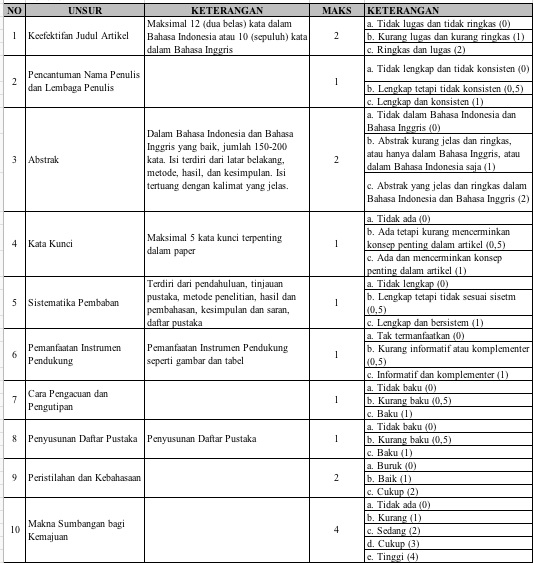
\includegraphics[width=1\textwidth]
      {figures/form1}}
      \caption{Form nilai bagian 1.}
      \label{form1}
      \end{figure}

	\begin{figure}[ht]
	      \centerline{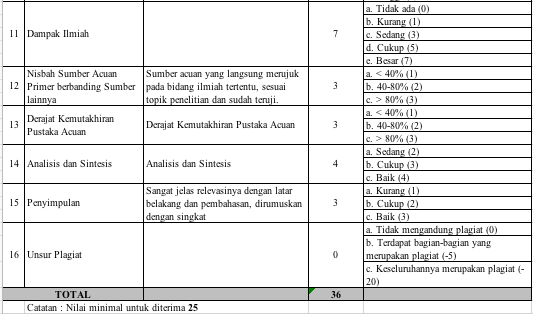
\includegraphics[width=1\textwidth]
	      {figures/form2}}
	      \caption{form nilai bagian 2.}
	      \label{form2}
	      \end{figure}

\chapter{FAQ}

M : Kalo Intership II atau TA harus buat aplikasi ?
D : Ga harus buat aplikasi tapi harus ngoding

M : Pa saya bingung mau ngapain, saya juga bingung mau presentasi apa?
D : Makanya baca de, buka jurnal topik `ganteng' nah kamu baca dulu sehari 5 kali ya, 4 hari udah 20 tuh. Bingung itu tanda kurang wawasan alias kurang baca.

M : Pa saya sudah cari jurnal terindeks scopus tapi ga nemu.
D : Kamu punya mata de? coba dicolok dulu. Kamu udah lakuin apa aja? tolong di list laporkan ke grup Tingkat Akhir. Tinggal buka google scholar klik dari tahun 2014, cek nama jurnalnya di scimagojr.com beres.

M : Pa saya belum dapat tempat intership, jadi ga tau mau presentasi apa?
D : kamu kok ga nyambung, yang dipresentasikan itu yang kamu baca bukan yang akan kamu lakukan.

M : Pa ini jurnal harus yang terindex scopus ga bisa yang lain ?
D : Index scopus menandakan artikel tersebut dalam standar semantik yang mudah dipahami dan dibaca serta bukan artikel asal jadi. Jika diluar scopus biasanya lebih sukar untuk dibaca dan dipahami karena tidak adanya proses review yang baik dan benar terhadap artikel.

M : Pa saya tidak mengerti
D : Coba lihat standar alasan

M : Pa saya bingung
D : Coba lihat standar alasan

M : Pa saya sibuk
D : Mbahmu....

M : Pa saya ganteng
D : Ndasmu....

M : Pa saya kece
D : wes karepmu lah....


Biasanya anda memiliki alasan tertentu jika menghadapi kendala saat proses bimbingan, disini saya akan melakukan standar alasan agar persepsi yang diterima sama dan tidak salah kaprah. Penggunaan kata alasan tersebut antara lain :

1. Tidak Mengerti : anda boleh menggunakan alasan ini jika anda sudah melakukan tahapan membaca dan meresumekan 15 jurnal. Sudah mencoba dan mempraktekkan teorinya dengan mencari di youtube dan google minimal 6 jam sehari selama 3 hari berturut-turut.

2. Bingung : anda boleh mengatakan alasan bingung setelah maksimal dalam berusaha menyelesaikan tugas bimbingan dari dosen(sudah dilakukan semua). Anda belum bisa mengatakan alasan bingung jika anda masih belum menyelesaikan tugas bimbingan dan poin nomor 1 diatas. Setelah anda menyelesaikan tugas bimbingan secara maksimal dan tahap 1 poin diatas, tapi anda masih tetap bingung maka anda boleh memakai alasan ini.

%next line adds the Bibliography to the contents page

%uncomment next line to change bibliography name to references
%\renewcommand{\bibname}{References}
\bibliography{references}        %use a bibtex bibliography file refs.bib
\bibliographystyle{plain}  %use the plain bibliography style

\end{document}

